% !TEX root = ../dissertacao.tex
\chapter{Resultados Experimentais}
\label{cap:resultados}

Este capítulo apresenta os resultados experimentais obtidos por este trabalho. 
Inicialmente, a Seção~\ref{sec:metodologia_experimental} descreve a metodologia adotada para avaliar os modelos de programação \ac{ood} e \ac{dod}.
A Seção~\ref{sec:infraestrutura_experimental} apresenta a infraestrutura experimental utilizada.
Por fim, as Seções~\ref{sec:estudo_de_caso_1} a \ref{sec:estudo_de_caso_4} apresentam um detalhamento de cada estudo de caso pertencente.
Para cada estudo de caso é apresentado seu algoritmo, suas organizações de dados e é realizada uma análise dos resultados experimentais obtidos.


\section{Metodologia Experimental}
\label{sec:metodologia_experimental}

Para quantizar o impacto da organização dos dados, foram avaliados o \textbf{número de  \textit{cache misses}} e o \textbf{tempo de execução} para cada um dos estudos de caso definidos no Capítulo~\ref{cap:caracterizacaoSinteseFisica}.
Para os estudos de caso 1, 2, e 3 foram implementadas quatro versões: 1) utilizando o modelo \ac{ood} com execução sequencial; 2) utilizando o modelo \ac{dod} com execução sequencial; 3) utilizando o modelo \ac{ood} com execução paralela; 4) utilizando o modelo \ac{dod} com execução paralela.
Para o estudo de caso 4 foram implementadas 2 versões: 1) utilizando o modelo \ac{ood} com execução sequencial; 2) utilizando o modelo \ac{dod} com execução sequencial.
Devido às interferências causadas pelo sistema operacional, os experimentos podem apresentar resultados diferentes em cada execução.
Assim, para aumentar a confiança estatística obtida, os experimentos foram repetidos 30 vezes, o que resultou em 99\% de confiança estatística\footnote{A confiança estatística foi medida utilizando o teste t de Student para p=0,01.}. Os resultados apresentados neste capítulo são as médias de 30 execuções.


\section{Infraestrutura e configuração experimental}
\label{sec:infraestrutura_experimental}

Os experimentos realizados utilizaram como entradas o conjunto de benchmarks disponibilizados pela competição \textit{ICCAD 2015 CAD Contest (problema C: Incremental Timing-Driven Placement)} \cite{kim2015}, o qual inclui 8 circuitos que possuem entre 768k e 1,93M células, todos derivados de circuitos industriais. Optou-se por utilizar tal infraestrutura pois a mesma disponibiliza circuitos com número de células compatível com circuitos contemporâneos. Além disso, tal infraestrutura é de acesso aberto, o que facilita a comparação experimental deste trabalho com trabalhos futuros. Como biblioteca básica, utilizou-se a Ophidian: Open-Source Library for Physical Design Research and Teaching~\cite{ophidian}.

Todas as implementações foram realizadas na linguagem $C++$ e compiladas com o compilador GCC 5.4.0. Para compilações com otimizações foram utilizadas as \textit{flags}: $O3$, ftree-vectorize e fopenmp. A \textit{flag} ftree-vectorize é responsável por habilitar a vetorização do código compilado, enquanto a \textit{flag} fopenmp é responsável pela paralelização do código com a biblioteca OpenMP~\cite{openmp}. Para medição do número de  \textit{cache misses} foi utilizada a ferramenta PAPI~\cite{papi} $5.6.0$.

Todos os experimentos foram executados em um computador com sistema operacional Debian GNU/Linux $8.2$ e processador Intel\textsuperscript{\textregistered} Core\textsuperscript{\textregistered} i5-4460 CPU @ 3.20~GHz.
A Figura~\ref{fig:architectureMemoryZeus} apresenta de forma gráfica a arquitetura deste computador.
Este computador possui 32GB RAM (DDR3 @ 1600MHz) como memória principal.
Seu processador possui quatro núcleos idênticos e três níveis de \textit{cache}.
Os primeiros dois níveis de \textit{cache}~(L1 and L2) são privativos para cada core do processador e possuem 64KB e 256KB de capacidade, respectivamente.
O terceiro nível de \textit{cache}~(L3) é compartilhado e possui 6144KB de capacidade.
Este processador possui $11$ contadores de \textit{hardware}, o que possibiliza à ferramenta PAPI analisar os três níveis de \textit{cache} simultaneamente.

\begin{figure}[ht]
    \centering
    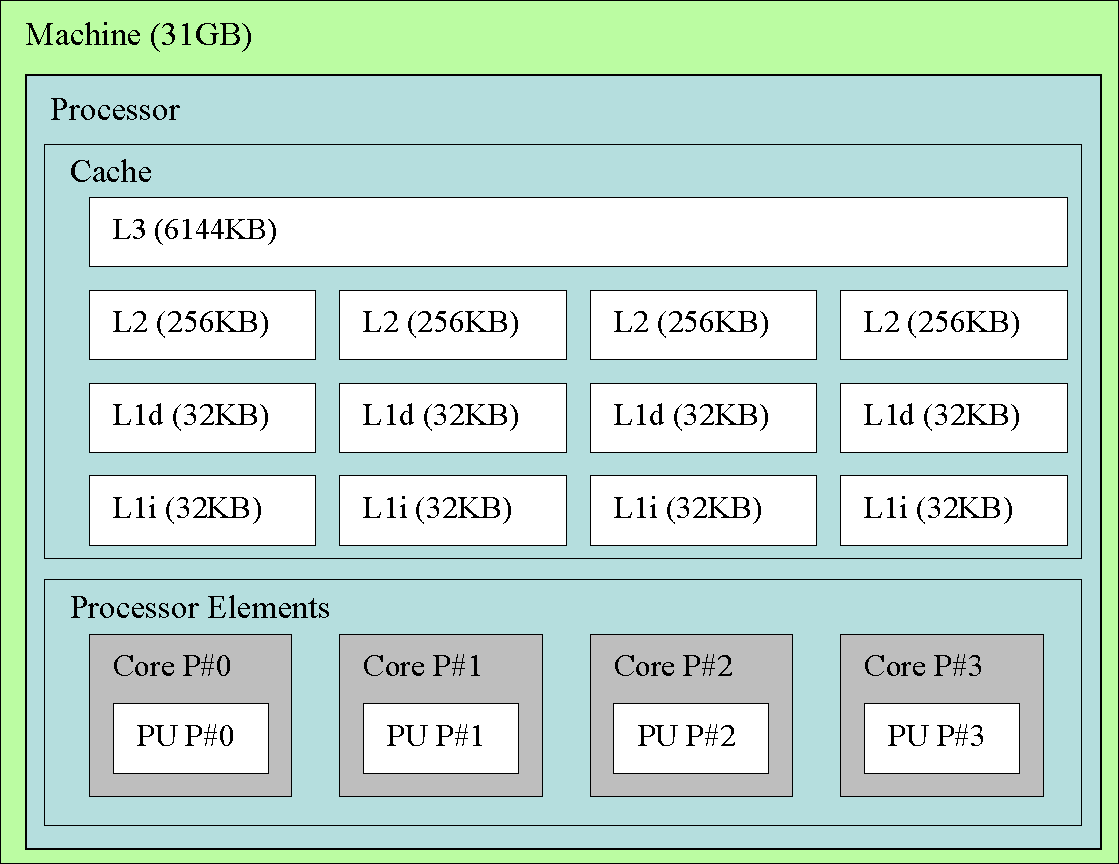
\includegraphics[width=0.5\linewidth]{img/results/architectureMemoryZeus.pdf}
    \caption{Arquitetura do computador utilizado nos experimentos.}
    \label{fig:architectureMemoryZeus}
\end{figure}


\section{Estudo de caso 1: Verificando os Limites do Chip}
\label{sec:estudo_de_caso_1}

Este estudo de caso visa avaliar um problema com baixa intensidade aritmética sobre um grande conjunto de dados.
Este problema consiste em verificar se cada célula do circuito está contida dentro dos limites físicos do \ac{ic}, estando presente na etapa de legalização do circuito.
Como a legalização é executada inúmeras vezes no fluxo de projeto é essencial que esta seja o mais otimizada possível.
Portanto, esta verificação pode impactar no desempenho da etapa de legalização pertencente à síntese física.

O Algoritmo~\ref{alg:problem1} descreve os passos a serem executados para verificar se todas as células estão posicionadas dentro dos limites de um chip.
Este Algoritmo recebe como entrada um conjunto de células $C$ e os limites do chip. 
Cada célula $c_i \in C$ possui sua localização representada por um ponto $(x(c_i), y(c_i))$.
Os limites do chip são representados por uma quádrupla ($\mathcal{X}_{min}$, $\mathcal{X}_{max}$ , $\mathcal{Y}_{min}$, $\mathcal{Y}_{max}$), onde $\mathcal{X}_{min}$ e  $\mathcal{Y}_{min}$ denotam os limites inferiores; e $\mathcal{X}_{max}$ e $\mathcal{Y}_{max}$ retratam os limites superiores.
Inicialmente, uma variável que representa quantas células existem fora dos limites do chip é inicializada com zero (linha \ref{alg:problem1:var:initIlegal}).
Então, para cada célula $c_i$ do circuito (linhas \ref{alg:problem1:var:initFor} a \ref{alg:problem1:var:endFor}) é analisada se sua posição encontra-se fora dos limites (linhas \ref{alg:problem1:var:if}).
Se a posição de $c_i$ estiver além dos limites do chip a variável $ilegal$ é incrementada (linha \ref{alg:problem1:var:atribuicao}).
O número de células que estão fora dos limites do chip é retornado após percorrer todas as células (linha \ref{alg:problem1:var:retorno}).

\simbolo{$C$}{conjunto de células $C$ do circuito}
\simbolo{$c_i$}{i-ésima célula do conjunto $C$}
\simbolo{$x(c_i)$}{posição no eixo $x$ da célula $c_i$}
\simbolo{$y(c_i)$}{posição no eixo $y$ da célula $c_i$}

\begin{algorithm}[h!t]
	\SetKwInOut{Input}{Entrada}\SetKwInOut{Output}{Saída}
	\LinesNumbered
  	\Input{Conjunto de células $C$, Limites do Chip ($\mathcal{X}_{min}$, $\mathcal{X}_{max}$ , $\mathcal{Y}_{min}$, $\mathcal{Y}_{max}$) }
  	\Output{ Número de células além dos limites do chip }
    $ilegal \gets 0$\; \label{alg:problem1:var:initIlegal}
  	\ForEach{$c_i \in C$}{ \label{alg:problem1:var:initFor}
  	    \uIf{$(x(c_i) < \mathcal{X}_{min}) \lor (x(c_i) > \mathcal{X}_{max}) \lor$ $(y(c_i) < \mathcal{Y}_{min}) \lor (y(c_i) > \mathcal{Y}_{max})$}{ \label{alg:problem1:var:if}
  	       $ilegal \gets ilegal + 1$\; \label{alg:problem1:var:atribuicao}
  	    }
  	} \label{alg:problem1:var:endFor}
  	\Return $ilegal$\; \label{alg:problem1:var:retorno}
	\caption{Verificação dos Limites do Chip} 
	\label{alg:problem1}
\end{algorithm}

Na Figura~\ref{fig:problem1} estão representados dois exemplos de posicionamento de células em um circuito.
A única diferença entre estes posicionamentos (Figura~\ref{subfig:problem1_a} e  \ref{subfig:problem1_b}) é o posicionamento da célula $c_1$.
No posicionamento da Figura~\ref{subfig:problem1_a} a célula $c_1$ viola o limite esquerdo do chip ($\mathcal{X}_{min}$), o que torna necessário executar algoritmos de legalização sobre este posicionamento para que a célula $c_1$ seja relocada para uma posição válida e legal.

\begin{figure}[ht]
    \centering
    \subfigure[Circuito com células além do limite do chip.]{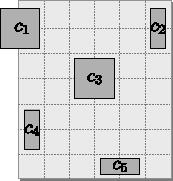
\includegraphics[width=0.33\linewidth]{img/results/problem1/problem1_a.pdf} \label{subfig:problem1_a}}
    \hspace{1cm}
    \subfigure[Circuito sem violação dos limites do chip.]{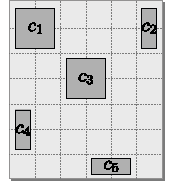
\includegraphics[width=0.33\linewidth]{img/results/problem1/problem1_b.pdf} \label{subfig:problem1_b}}
    \caption{Exemplo de posicionamento de células sobre um circuito.}
    \label{fig:problem1}
\end{figure}

\subsection{Modelagem dos Dados}

Para verificar se todas as células estão contidas dentro dos limites do chip são necessárias três informações: limites do chip, lista das células e a posição de cada célula.
Estas informações podem ser separadas em três módulos: \textit{Floorplan}, \textit{Netlist} e \textit{Placement}.
O módulo \textit{Floorplan} contém informações pertinentes a área do circuito, como limites do chip e tamanho das linhas e colunas.
O módulo \textit{Netlist}, por sua vez, representa as informações das interconexões e lista das células do circuito.
No módulo \textit{Placement} estão contidas informações do posicionamento e geometrias das células.
Portanto, é possível modelar o problema utilizando \ac{ood} com três classes: \textit{Floorplan::Floorplan, Netlist::Cell e Placement::Cell}.
A Figura~\ref{subfig:problem1ModelagemDados_OOD} apresenta o diagrama de classes para este modelo de programação.
A seta entre as classes \textit{Cell} dos módulos \textit{Netlist} e \textit{Placement} representa uma relação de hierarquia, significando que a classe \textit{Cell} do módulo \textit{Placement} estende os atributos da classe \textit{Cell} do módulo \textit{Netlist}.

\begin{figure}[h!t]
    \centering
    \subfigure[]{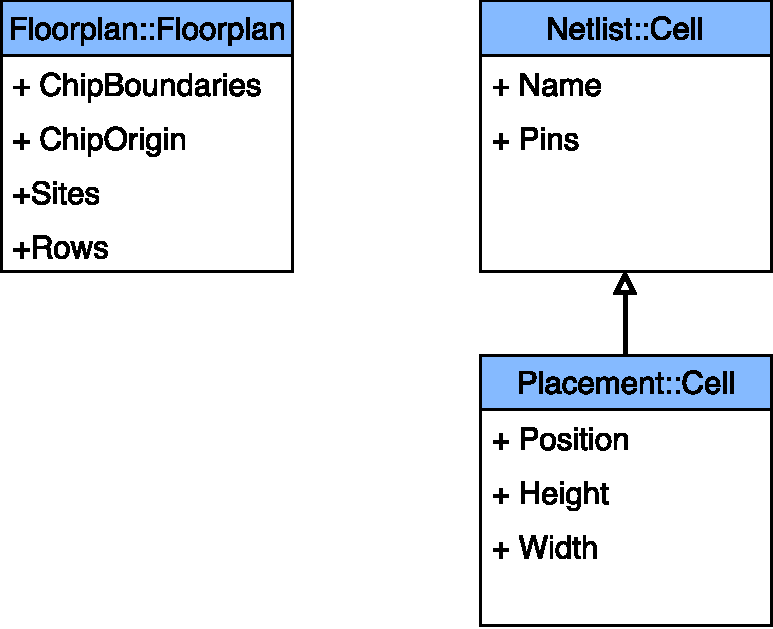
\includegraphics[width=0.6\linewidth]{img/results/problem1/classHierarchyChipBoundariesOOD.pdf} \label{subfig:problem1ModelagemDados_OOD}}
    % \hspace{0.1cm}
    
    \subfigure[]{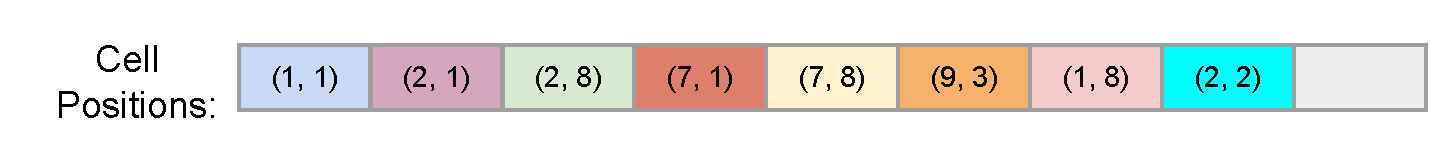
\includegraphics[width=0.9\linewidth]{img/results/problem1/chipBoundariesDOD.pdf} \label{subfig:problem1ModelagemDados_DOD}}
    \caption[Organização dos dados estudo de caso 1]{Organização dos dados para o problema de verificação dos limites do chip segundo os modelos de programação OOD (a) e DOD (b).}
    \label{fig:problem1ModelagemDados}
\end{figure}

Com esta abordagem dos dados, segundo o modelo \ac{ood}, pode-se perceber que existem atributos nos objetos que não serão utilizados por este problema (nome e pinos pertencentes a uma célula).
Porém, estes atributos serão recuperados juntamente com atributos úteis para o problema.
Tal comportamento pode reduzir a localidade espacial do programa e por consequência, degradar o desempenho da aplicação de modo geral.

Adotando o modelo de programação \ac{dod}, são necessárias somente duas informações: limites do chip e a posição de cada célula.
A Figura~\ref{subfig:problem1ModelagemDados_DOD} apresenta um possível organização dos dados segundo este modelo de programação.
As posições de todas as células são armazenadas contiguamente em um único vetor (\textit{Cell  Positions}), o que evita a necessidade de uma lista com todas as células pertencentes ao chip.
Neste modelo de dados, o laço presente na linha \ref{alg:problem1:var:initFor} do Algoritmo~\ref{alg:problem1} seria limitado a percorrer todos os dados contidos no vetor \textit{Cell  Positions}.
Esta abordagem conduz a uma exploração adequada da localidade espacial para este algoritmo e também reduz o número de atributos necessários para a sua execução.

\subsection{Avaliação}

A Figura~\ref{fig:problem1resultSequencial} apresenta os resultados da execução sequencial da verificação dos limites do chip.
Na Figura~\ref{fig:missSequentialProblem1} são apresentados os números de \textit{cache misses} (eixo Y), em escala logarítmica, para cada circuito avaliado (eixo X).
Para cada circuito, a entrada considerada corresponde ao conjunto de todas as células do circuito.
As barras amarelas representam o modelo de dados Orientado a Objetos (\ac{ood}), ao passo que as barras azuis representam o modelo Orientado a Dados (\ac{dod}). O número total de  \textit{cache misses} para o \ac{dod} (de $87$ a $103$) foi, em média, cinco ordens de grandeza menor do que aquele resultante da aplicação do modelo \ac{ood} (de $3M$ a $11M$). A redução no número de  \textit{cache misses} é proveniente diretamente da melhor organização dos dados em memória. Nesta organização, os dados de uma mesma propriedade (posição de uma determinada célula, neste problema) estão armazenados contiguamente em memória. Portanto, ao ocorrer um miss na \textit{cache}, somente dados úteis são recuperados da memória principal. Assim, é realizado um melhor aproveitamento dos blocos de dados recuperados da memória principal para a \textit{cache}.
Outro fator importante é a vetorização do código gerado pelo compilador. Como o laço (linha \ref{alg:problem1:var:initFor} a \ref{alg:problem1:var:endFor} do Algoritmo~\ref{alg:problem1} para modelo \ac{dod}) acessa somente informações contidas em um vetor, o compilador consegue facilmente identificar esse comportamento e substituir as instruções padrão (\ac{sisd}) por instruções vetoriais (\ac{simd}).

\begin{figure}[h!b]
    \centering
    \subfigure[Número de  \textit{cache misses}.]{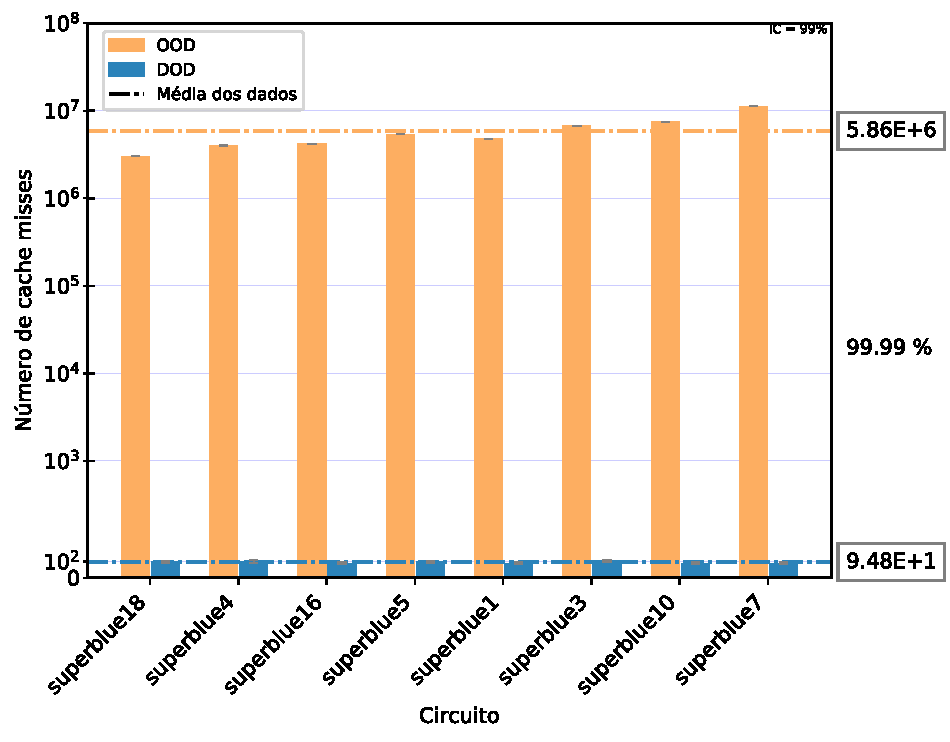
\includegraphics[width=0.47\linewidth]{img/results/problem1/problem1_miss_sequential.pdf} \label{fig:missSequentialProblem1}}
    \subfigure[Tempo de execução.]{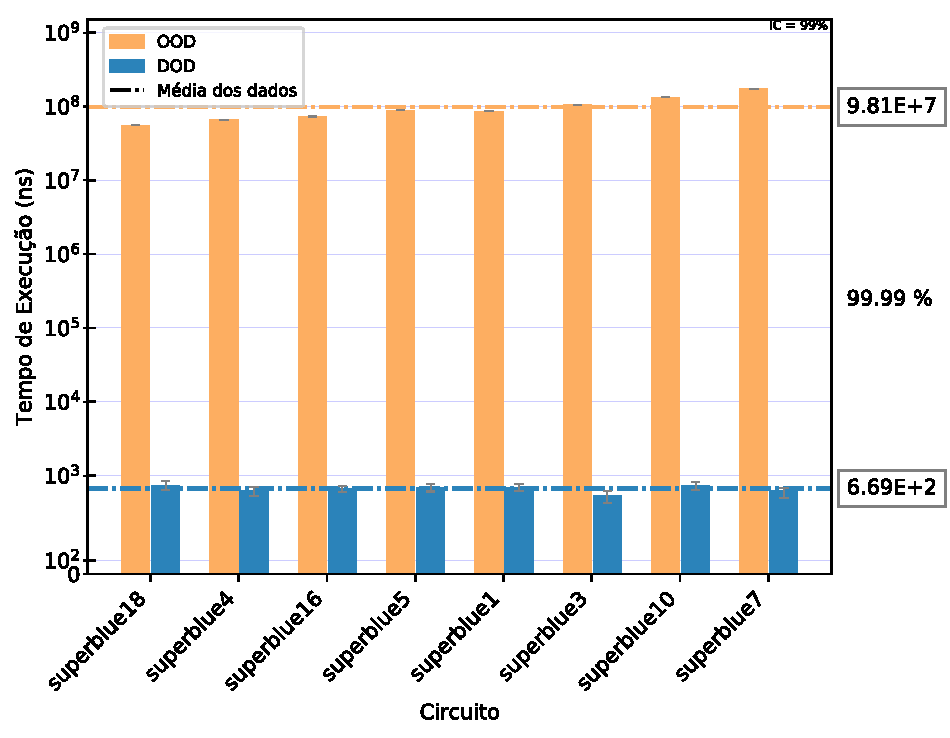
\includegraphics[width=0.47\linewidth]{img/results/problem1/problem1_runtime_sequential.pdf} \label{fig:runtimeSequentialProblem1}}
    \caption{Resultados experimentais para a execução sequencial do estudo de caso 1.}
    \label{fig:problem1resultSequencial}
\end{figure}

% \begin{figure}[ht]
%     \centering
%     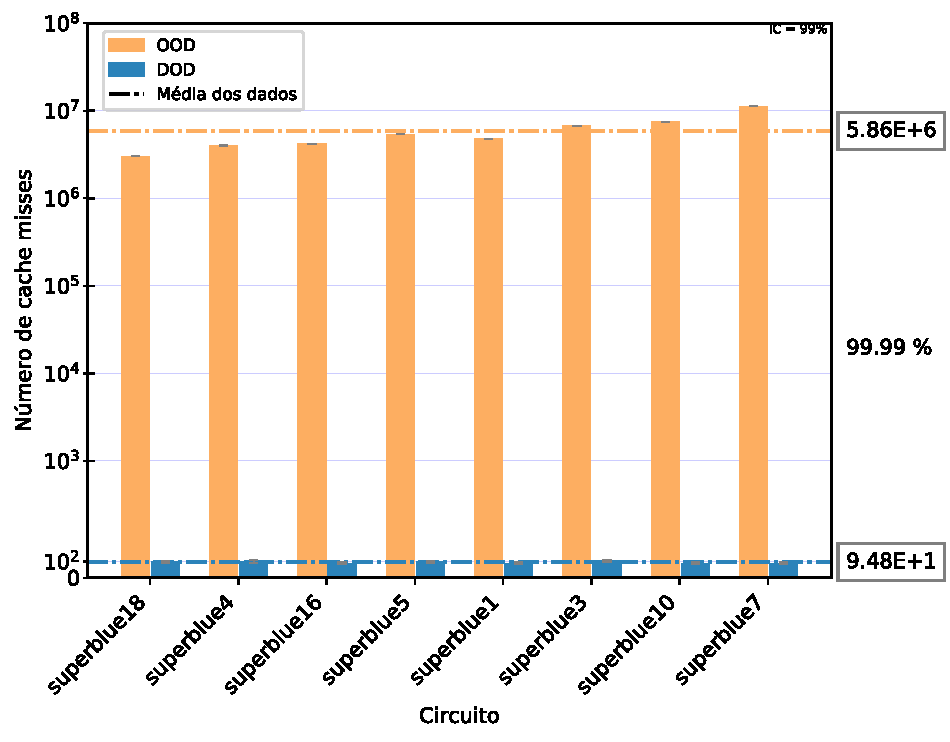
\includegraphics[width=0.65\linewidth]{img/results/problem1/problem1_miss_sequential.pdf}
%     \caption[Cache misses do estudo de caso~1 sequencial.]{Número de cache misses resultantes dos dois protótipos de software do studo de caso~1 com execução sequencial.}
%     \label{fig:missSequentialProblem1}
% \end{figure}

A exploração da localidade dos dados reduz o tempo de acesso à memória principal, que constitui o gargalo principal. O impacto desta redução no tempo de execução pode ser observado na Figura~\ref{fig:runtimeSequentialProblem1}. Este gráfico, em escala logarítmica, retrata o tempo de execução (eixo Y) em nanossegundos para cada circuito avaliado (eixo X). Pode-se observar que a versão \ac{dod} executou mais rápido em todos os circuitos avaliados. Os tempos de execução da versão \ac{dod} estão entre $572ns$ e $743ns$, enquanto os tempos de execução de \ac{ood} estão entre $55ms$ e $174ms$.
Note que a implementação com \ac{dod} executou em \textbf{nanossegundos} ao invés de \textbf{milissegundos}, correspondendo a uma redução média de cinco ordens de grandeza.
Portanto, para o estudo de caso~1, a diferença relativa~\footnote{A diferença relativa foi calculada com a seguinte equação: $dr = \frac{(OOD - DOD)}{OOD}$, onde OOD e DOD representam a média da métrica avaliada (número de  \textit{cache misses} ou tempo de execução).} entre a modelagem dos dados com \ac{ood} e com \ac{dod} é de $99.99\%$, em média.

% \begin{figure}[ht]
%     \centering
%     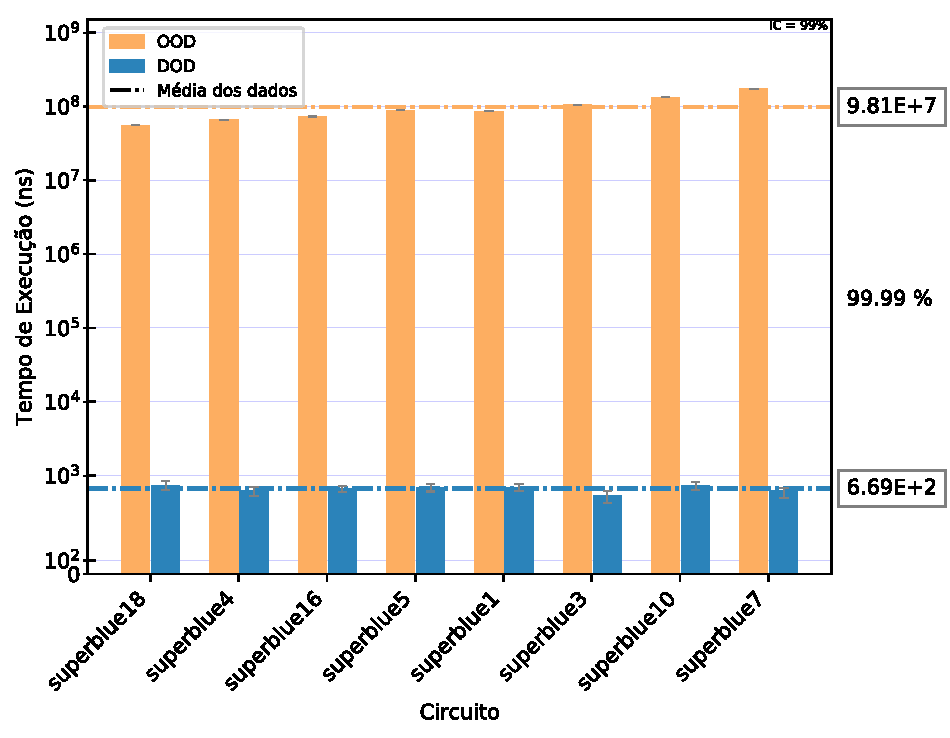
\includegraphics[width=0.65\linewidth]{img/results/problem1/problem1_runtime_sequential.pdf}
%     \caption[Tempo de execução estudo de caso~1 sequencial]{Tempo de execução para o estudo de caso~1 com execução sequencial.}
%     \label{fig:runtimeSequentialProblem1}
% \end{figure}

O Algoritmo~\ref{alg:problem1paralelo} apresenta uma versão paralela do Algoritmo~\ref{alg:problem1}.
Neste algoritmo o conjunto de células é percorrido de forma simultânea por diferentes \textit{threads}.
Note que a variável $ilegal$ deve ser compartilhada entre todos os fluxos de execução e pode ser escrita simultaneamente.
Para isso, a função $reduction$, da API OpenMP~\cite{openmp}, fornece a cada \textit{thread} uma cópia local da variável $ilegal$ e, ao final de todos os fluxos de execuções, sincroniza o valor da variável de forma exclusiva.


\begin{algorithm}[h!t]
	\SetKwInOut{Input}{Entrada}\SetKwInOut{Output}{Saída}
	\LinesNumbered
  	\Input{Conjunto de células $C$, Limites do Chip ($\mathcal{X}_{min}$, $\mathcal{X}_{max}$ , $\mathcal{Y}_{min}$, $\mathcal{Y}_{max}$) }
  	\Output{ Número de células além dos limites do chip }
    $ilegal \gets 0$\; \label{alg:problem1paralelo:var:initIlegal}
  	\textit{\textbf{\#pragma omp parallel for reduction(}}$+:ilegal$\textit{\textbf{)}} \hspace{20pt} \ForEach{$c_i \in C$}{ \label{alg:problem1paralelo:var:initFor}
  	    \uIf{$(x(c_i) < \mathcal{X}_{min}) \lor (x(c_i) > \mathcal{X}_{max}) \lor$ $(y(c_i) < \mathcal{Y}_{min}) \lor (y(c_i) > \mathcal{Y}_{max})$}{ \label{alg:problem1paralelo:var:if}
  	       $ilegal \gets ilegal + 1$\; \label{alg:problem1paralelo:var:atribuicao}
  	    }
  	} \label{alg:problem1paralelo:var:endFor}
  	\Return $ilegal$\; \label{alg:problem1paralelo:var:retorno}
	\caption{Verificação dos Limites do Chip em Paralelo} 
	\label{alg:problem1paralelo}
\end{algorithm}

A Figura~\ref{fig:problem1ExecParallel} apresenta os resultados obtidos com a execução paralela do estudo de caso~1.
Na esquerda (Figura~\ref{fig:problem1ExecParallelMiss}) é apresentado, em escala logarítmica, o número de  \textit{cache misses} (eixo Y) para cada circuito (eixo X).
O número de  \textit{cache misses} para o modelo \ac{ood} foi entre $1M$ a $6M$ enquanto, para o modelo \ac{dod} foi entre $83k$ a $202k$.
Esta redução foi, em média, de uma ordem de grandeza.
No lado direito (Figura~\ref{fig:problem1ExecParallelRuntime}) é apresentado, em escala logarítmica, o tempo de execução em nanossegundos (eixo Y) para cada circuito (eixo X).
O tempo de execução ficou entre $26$ e $96$ milissegundos para o modelo \ac{ood}. Já o modelo \ac{dod} executou entre $0.76$ e $1.62$ milissegundos, o que gerou uma redução média de uma ordem de grandeza e uma diferença relativa de $9.85\%$.

\begin{figure}[ht]
    \centering
    \subfigure[Número de  \textit{cache misses}.]{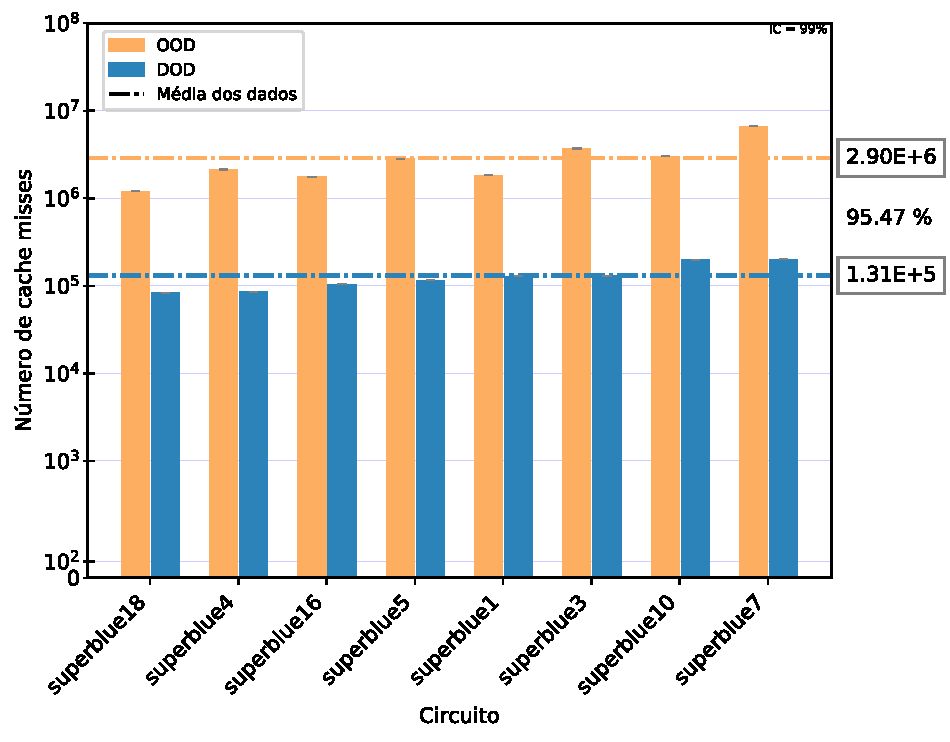
\includegraphics[width=0.48\linewidth]{img/results/problem1/problem1_miss_parallel.pdf} \label{fig:problem1ExecParallelMiss}}
    \subfigure[Tempo de execução.]{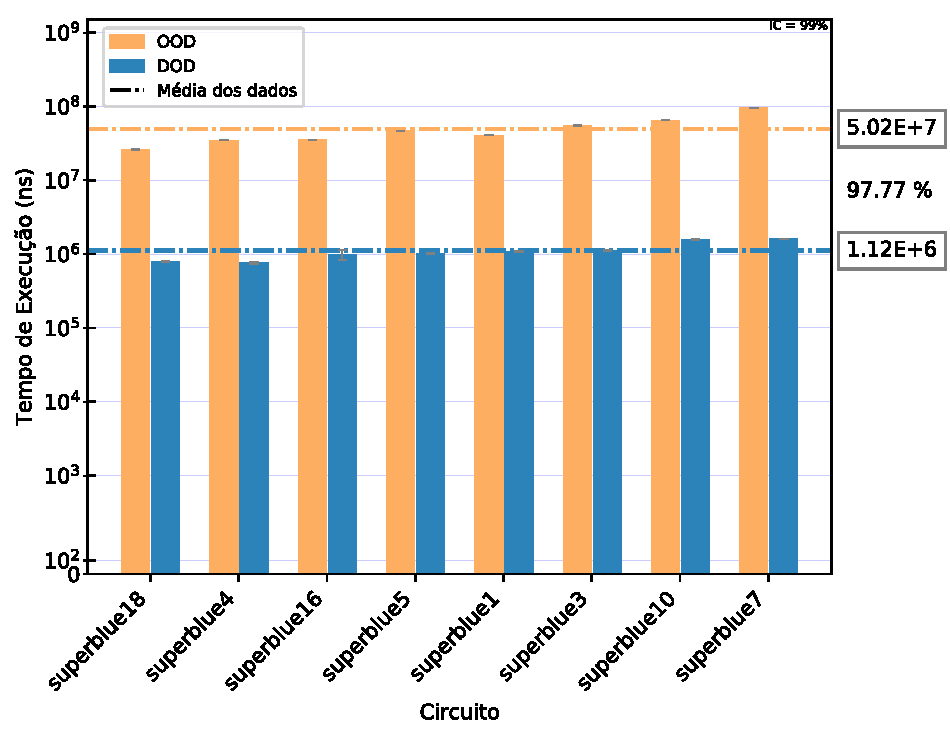
\includegraphics[width=0.48\linewidth]{img/results/problem1/problem1_runtime_parallel.pdf} \label{fig:problem1ExecParallelRuntime}}
    \caption[Resultados do estudo de caso~1 com execução paralela.]{Resultados, em escala logarítmica, para execução paralela do estudo de caso~1.}
    \label{fig:problem1ExecParallel}
\end{figure}

Comparando as execuções sequencial e paralela, pode-se notar que houve uma redução no número de  \textit{cache misses} para a versão \ac{ood} e um \textit{speedup} médio de $1.95$ no tempo de execução.
Porém, houve um aumento significativo no número de  \textit{cache misses} (aumento de 4 ordens de grandeza) e tempo de execução para a versão \ac{dod} (\textit{speedup} médio de $0.0006$).
Este aumento se deve ao fato de que a tarefa, no modelo \ac{dod}, já possuía um alto desempenho e seu tempo de execução era extremamente baixo.
O sobrecusto de criação e sincronização das \textit{threads} foi muito superior ao próprio tempo da aplicação.
Portanto, a paralelização desta aplicação não apresentou ganhos significativos quando comparado com a versão sequencial.


% \begin{figure}[ht]
%     \centering
%     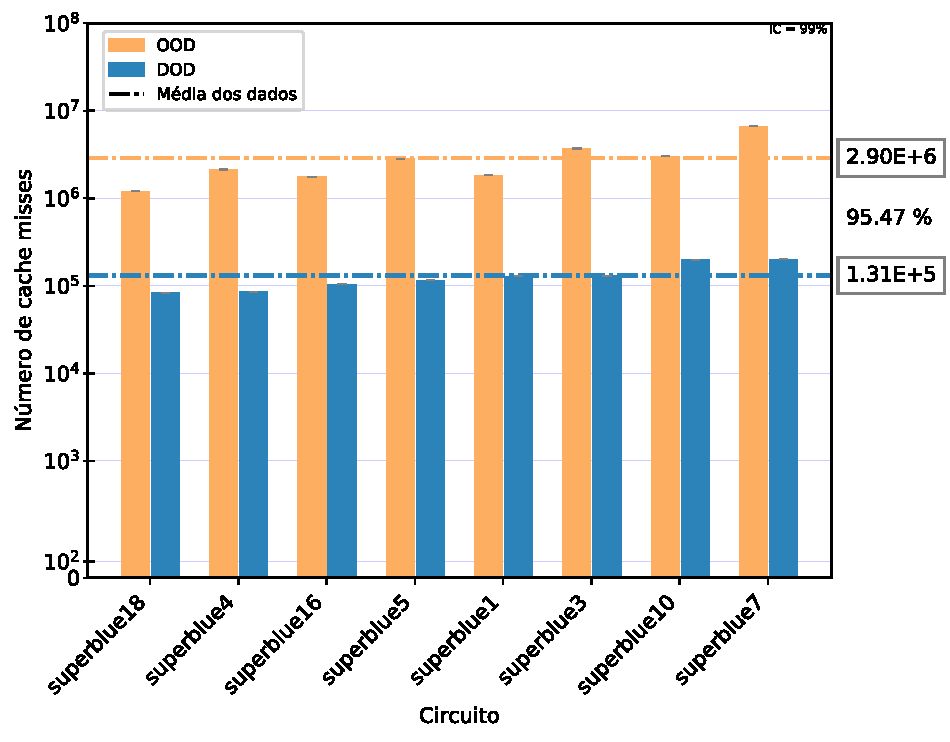
\includegraphics[width=0.65\linewidth]{img/results/problem1/problem1_miss_parallel.pdf}
%     \caption[Cache misses do Problema~1 paralelo.]{Número de cache misses resultantes dos dois protótipos de software do Problema~1 com execução paralela.}
%     \label{fig:missParallelProblem1}
% \end{figure}

% \begin{figure}[ht]
%     \centering
%     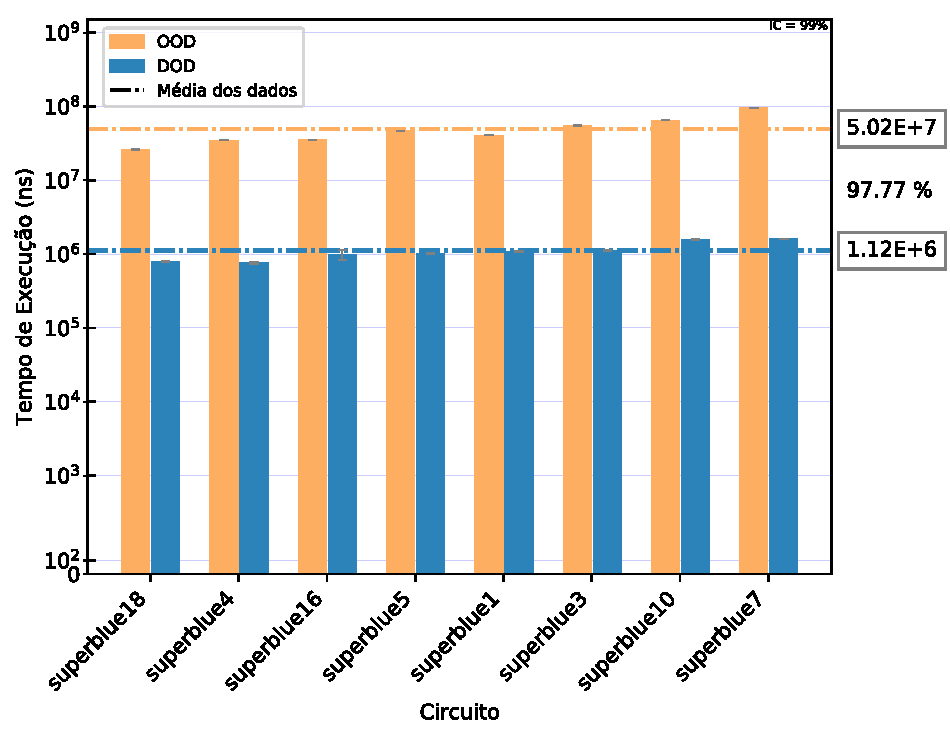
\includegraphics[width=0.65\linewidth]{img/results/problem1/problem1_runtime_parallel.pdf}
%     \caption[Tempo de execução Problema~1 paralelo]{Tempo de execução para o Problema~1 com execução paralela.}
%     \label{fig:runtimeParallelProblem1}
% \end{figure}









\section{Estudo de caso 2: Estimativa do Comprimento de Interconexões}
\label{sec:estudo_de_caso_2}

A proposta deste estudo de caso é avaliar uma tarefa de baixa intensidade aritmética porém, com necessidade de diversas propriedades de diferentes entidades.
A estimativa das interconexões, dentro da síntese física, é uma atividade utilizada por algoritmos de posicionamento e \textit{timing/power optimization}.
Exitem diversos métodos para estimar o comprimento de uma interconexão, dentre eles estão o \ac{rsmt} e \ac{hpwl}.
A \ac{rsmt} fornece estimativas de comprimento com um alto nível de precisão, porém possui complexidade computacional superior a do \ac{hpwl}.

O modelo \ac{hpwl} é comumente usado nas etapas iniciais da síntese física por possuir um tempo de execução linear com relação ao número de pinos pertencentes à interconexão ($\mathcal{O}|Pins|$).
O comprimento de fio é estimado como a metade do perímetro do retângulo mínimo que contém todos os pinos pertencentes a uma determinada interconexão.
A Figura~\ref{fig:problem2} exemplifica uma interconexão entre 4 células e seus respectivos pinos.
Na Figura~\ref{fig:problem2_a} é apresentada a \ac{rsmt} para esta interconexão, ao passo que na Figura~\ref{fig:problem2_b} é apresentada a estimativa \ac{hpwl} para a mesma interconexão.
Nesta, o retângulo mínimo que contém os quatro pinos possui perímetro de $18$ unidades. Portanto, o comprimento desta interconexão é estimado em $9$ unidades.

\begin{figure}[ht]
    \centering
    \subfigure[]{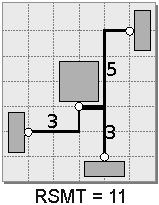
\includegraphics[width=0.25\linewidth]{img/results/problem2/problemaB_a.pdf} \label{fig:problem2_a}}
    \hspace{1cm}
    \subfigure[]{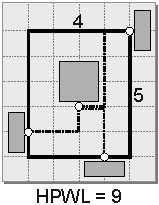
\includegraphics[width=0.25\linewidth]{img/results/problem2/problemaB_b.pdf} \label{fig:problem2_b}}
    \caption[Exemplo do cálculo de HPWL.]{Exemplo da estimativa do comprimento de uma interconexão de quatro pinos. Adaptada de \citeonline{kahng2011vlsi}.}
    \label{fig:problem2}
\end{figure}

O Algoritmo~\ref{alg:problem2} descreve o procedimento para o cálculo do \ac{hpwl} para todas as interconexões do \ac{ic}. 
Este algoritmo recebe como entrada um conjunto $N$ de todas as interconexões do \ac{ic} e retorna a estimativa do comprimento destas interconexões.
Inicialmente, a estimativa das interconexões ($hpwl$) é inicializada com zero (linha \ref{alg:problem2:var:inithpwl}).
Então, para cada interconexão $n_i$ pertencente ao conjunto $N$, o conjunto $P$ de seus pinos é recuperado (linha~\ref{alg:problem2:var:conjuntoPins}) e o retângulo que encapsula todos os pinos pertencentes a este conjunto é calculado (linhas~\ref{alg:problem2:var:initForPins} a \ref{alg:problem2:var:endForPins}).
Por conseguinte, a estimativa das interconexões ($hpwl$) do circuito é acrescida da metade do perímetro deste retângulo (linha~\ref{alg:problem2paralelo:var:somaHpwl}).
Finalmente, a estimativa total das interconexões é retornada na linha~\ref{alg:problem2:var:retorno}.

\simbolo{$N$}{conjunto de interconexões $N$ do circuito}
\simbolo{$n_i$}{i-ésima interconexão do conjunto $N$}
\simbolo{$pins(n_i)$}{\\ pinos pertencentes a interconexão $n_i$}
\simbolo{$P$}{conjunto de pinos $P$ do circuito}
\simbolo{$p_j$}{j-ésimo pino do conjunto $P$}
\simbolo{$x(p_j)$}{posição no eixo $x$ do pino $p_j$}
\simbolo{$y(p_j)$}{posição no eixo $y$ do pino $p_j$}

\begin{algorithm}[h!t]
	\SetKwInOut{Input}{Entrada}\SetKwInOut{Output}{Saída}
	\LinesNumbered
  	\Input{Conjunto de Interconexões do circuito $N$}
  	\Output{ Estimativa das Interconexões }
    $hpwl \gets 0$\; \label{alg:problem2:var:inithpwl}
  	\ForEach{$n_i \in N$}{ \label{alg:problem2:var:initForNets}
  	    $P \gets pins(n_i)$\; \label{alg:problem2:var:conjuntoPins}
  	    $x_{min}, y_{min} \gets \infty$\; \label{alg:problem2:var:initMin}
  	    $x_{max}, y_{max} \gets -\infty$\; \label{alg:problem2:var:initMax}
  	    \ForEach{$p_j \in P$}{ \label{alg:problem2:var:initForPins}
  	        \uIf{$x(p_j) < x_{min}$}{\label{alg:problem2:var:ifXmin} $x_{min} \gets x(p_j)$\;}
  	        \uIf{$y(p_j) < y_{min}$}{\label{alg:problem2:var:ifYmin} $y_{min} \gets y(p_j)$\;}
  	        \uIf{$x(p_j) > x_{max}$}{\label{alg:problem2:var:ifXmax} $x_{max} \gets x(p_j)$\;}
  	        \uIf{$y(p_j) > y_{max}$}{\label{alg:problem2:var:ifYmax} $y_{max} \gets y(p_j)$\;}
  	    } \label{alg:problem2:var:endForPins}
  	    $hpwl \gets hpwl + (x_{max} - x_{min}) + (y_{max} - y_{min})$\; \label{alg:problem2:var:somaHpwl}
  	} \label{alg:problem2:var:endForNets}
  	\Return $hpwl$\; \label{alg:problem2:var:retorno}
	\caption{\textit{Half-Perimeter Wirelength} (HPWL)} 
	\label{alg:problem2}
\end{algorithm}

\subsection{Modelagem dos Dados}
\label{subsec:modelagemDadosProblem2}

Para estimar o comprimento das interconexões utilizando o modelo \ac{hpwl} são necessárias três informações básicas a respeito do \ac{ic}: conjunto das interconexões, conjunto dos pinos pertencentes a cada interconexão, e posição dos pinos.
Estas informações podem ser divididas em dois módulos: \textit{Netlist} e \textit{Placement}.
A Figura~\ref{fig:problem2ModelagemDados} apresenta a organização dos dados para os modelos \ac{ood} e \ac{dod}.
Na Figura~\ref{subfig:problem2ModelagemDados_OOD} é apresentado o diagrama de classes para estimar uma interconexão seguindo o modelo de programação \ac{ood}.
Neste diagrama, a seta entre as classes \textit{Pin} dos módulos \textit{Netlist} e \textit{Placement} representa uma relação de hierarquia, ao passo que a seta com ponta em losango entre as classes \textit{Net} e \textit{Pin} representa uma relação de agregação --- o que significa que a \textit{Net} (interconexão) possui referência para seus \textit{pins} (pinos), enquanto os pinos possuem referência para sua interconexão.

Já para o modelo \ac{dod} são necessárias duas entidades (\textit{Nets} e \textit{Pins}) e duas propriedades (\textit{Net Pins} e \textit{Pins Position}), resultando em quatro vetores de informações. Estes vetores estão representados de forma gráfica na Figura~\ref{subfig:problem2ModelagemDados_DOD}.
Seguindo esta modelagem dos dados, o laço da linha~\ref{alg:problem2:var:initForNets} à \ref{alg:problem2:var:endForNets} do Algoritmo~\ref{alg:problem2:var:retorno} irá iterar sobre o vetor \textit{Nets} apresentado nesta figura. O conjunto de pinos $P$ acessado na linha~\ref{alg:problem2:var:conjuntoPins} será recuperado a partir do vetor \textit{Net Pins} deste modelo. Já o laço da linha~\ref{alg:problem2:var:initForPins} à \ref{alg:problem2:var:endForPins} irá percorrer o vetor \textit{Pins}.

\begin{figure}[ht]
    \centering
    % Diagrama de classes para modelar o problema de estimativa do comprimento de interconexões segundo paradigma de programação \ac{ood}.
    \subfigure[]{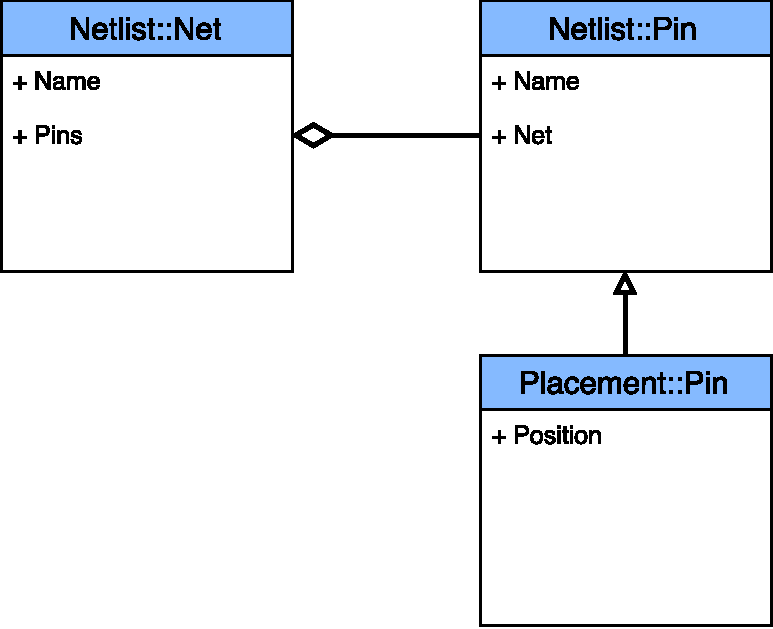
\includegraphics[width=0.3\linewidth]{img/results/problem2/classHierarchyOOD.pdf} \label{subfig:problem2ModelagemDados_OOD}}
    % \hspace{0.1cm}
    % Modelagem dos dados para o problema de estimativa do comprimento de interconexões segundo paradigma de programação \ac{dod}.
    \subfigure[]{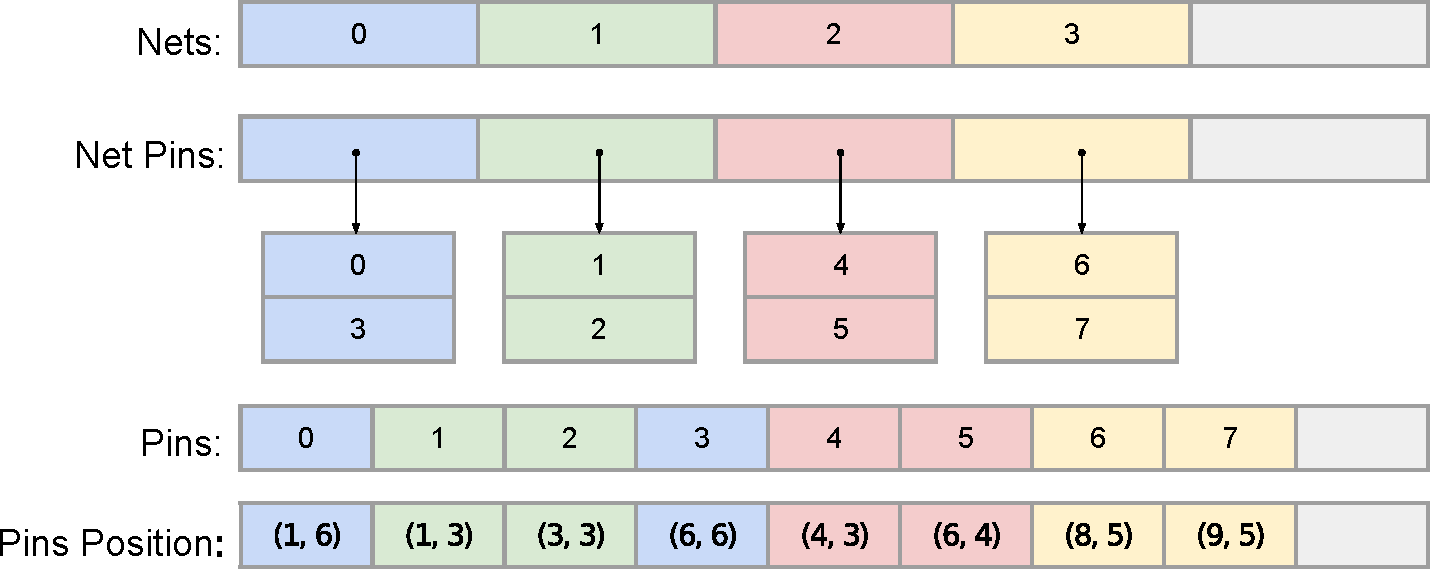
\includegraphics[width=0.64\linewidth]{img/results/problem2/estimativa_interconection_dod.pdf} \label{subfig:problem2ModelagemDados_DOD}}
    \caption[Organização dos dados estudo de caso 2]{Organização dos dados para estimativa de interconexões entre os modelos de programação OOD (a) e DOD (b).}
    \label{fig:problem2ModelagemDados}
\end{figure}


\subsection{Avaliação}

A Figura \ref{fig:problem2resultSequencial} apresenta os resultados para o estudo de caso 2 com execução sequencial. As barras amarelas representam o modelo de dados Orientado a Objetos (\ac{ood}), enquanto que as barras azuis representam o modelo Orientado a Dados (\ac{dod}). A Figura~\ref{fig:missSequentialProblem2} apresenta o número de  \textit{cache misses} (eixo Y) para cada circuito (eixo X). Para cada circuito, a entrada considerada corresponde ao conjunto de todas as interconexões do circuito.
O número de  \textit{cache misses} foi entre $8M$ e $20M$ para o modelo \ac{ood}, enquanto que o uso do modelo \ac{dod} resultou em $26M$ a $72M$.
A Figura~\ref{fig:runtimeSequentialProblem2} mostra o tempo de execução em milissegundos (eixo Y) para cada circuito (eixo X).
O modelo \ac{ood} executou entre $91$ e $226$ milissegundos, enquanto o modelo \ac{dod} executou entre $354$ e $951$ milissegundos 

\begin{figure}[ht]
    \centering
    \subfigure[Número de  \textit{cache misses}.]{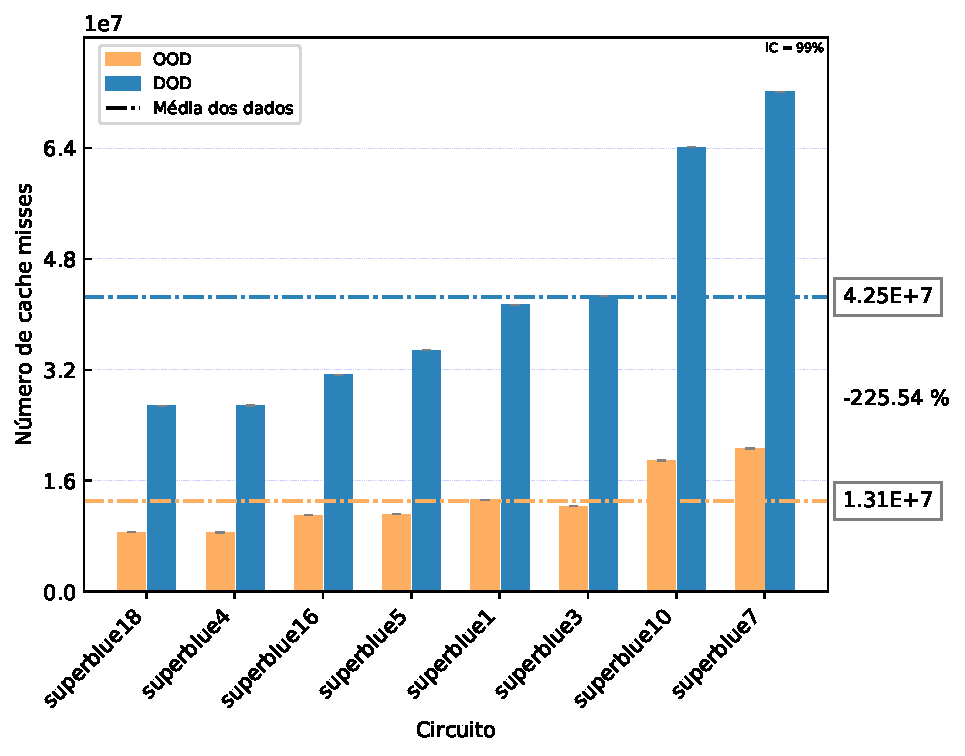
\includegraphics[width=0.47\linewidth]{img/results/problem2/problem2_miss_sequential.pdf} \label{fig:missSequentialProblem2}}
    % \hspace{1cm}
    \subfigure[Tempo de execução.]{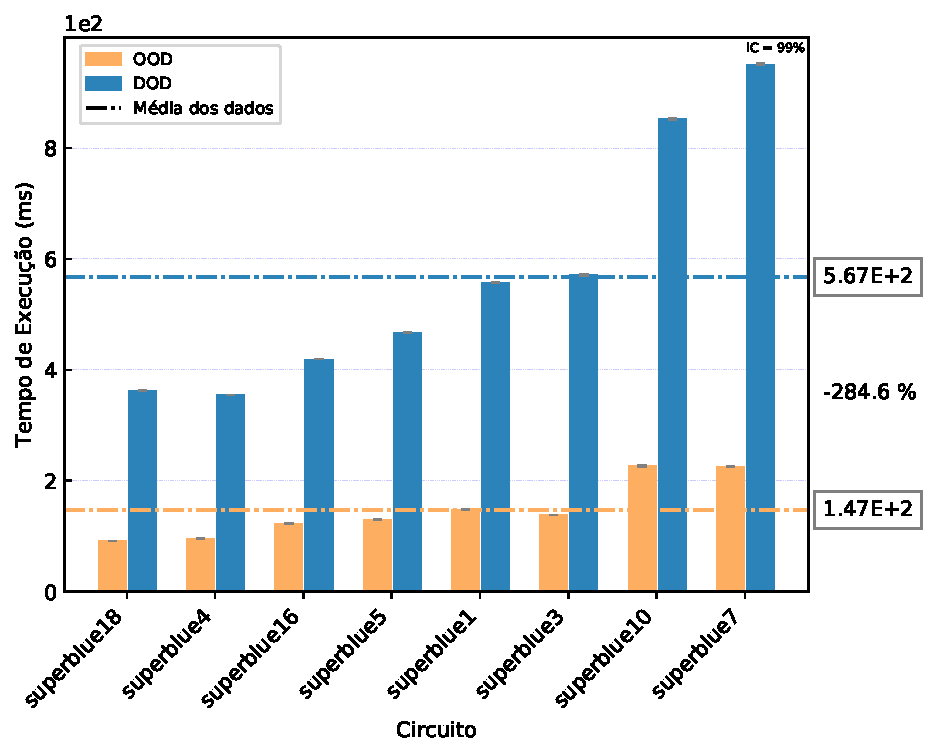
\includegraphics[width=0.47\linewidth]{img/results/problem2/problem2_runtime_sequential.pdf} \label{fig:runtimeSequentialProblem2}}
    \caption[Resultados estudo de caso 2 com execução sequencial]{Resultados com execução sequencial.}
    \label{fig:problem2resultSequencial}
\end{figure}

% \begin{figure}[ht]
%     \centering
%     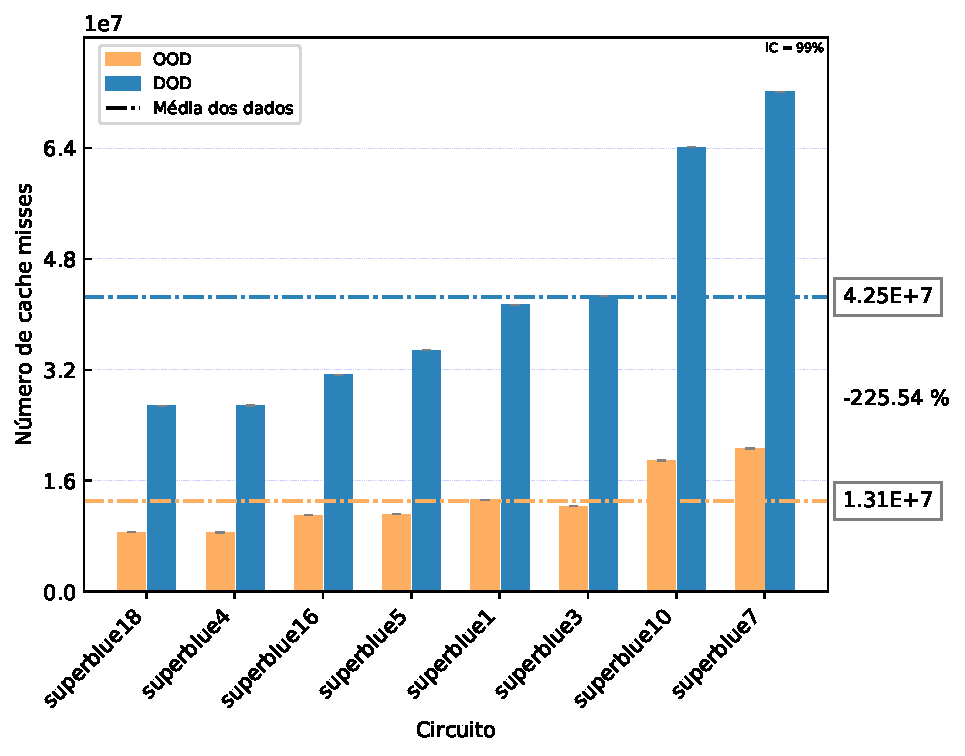
\includegraphics[width=0.65\linewidth]{img/results/problem2/problem2_miss_sequential.pdf}
%     \caption[Cache misses do Problema~2 sequencial.]{Número de cache misses resultantes dos dois protótipos de software do Problema~2 com execução sequencial.}
%     \label{fig:missSequentialProblem2}
% \end{figure}

% \begin{figure}[ht]
%     \centering
%     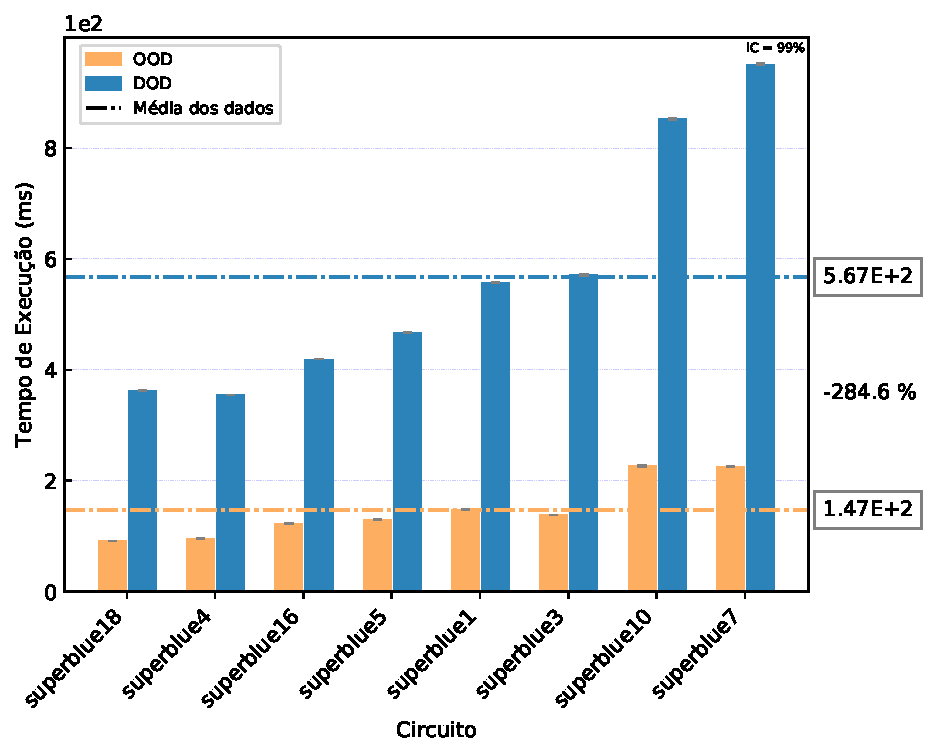
\includegraphics[width=0.65\linewidth]{img/results/problem2/problem2_runtime_sequential.pdf}
%     \caption[Tempo de execução Problema~2 sequencial]{Tempo de execução para o Problema~2 com execução sequencial.}
%     \label{fig:runtimeSequentialProblem2}
% \end{figure}

Na organização de dados considerada (e apresentada na Figura~\ref{fig:problem2ModelagemDados}), pode-se perceber que o modelo \ac{dod} resultou num número muito superior de  \textit{cache misses} do que o modelo \ac{ood}. Este número elevado de  \textit{cache misses} impactou diretamente em seu tempo total de execução.
Tal degradação de desempenho se deve ao fato de que a posição dos pinos no vetor \textit{Pin Positions} não reflete a ordem em que as interconexões serão percorridas (ordem do vetor \textit{Nets}). 
Este desalinhamento entre as ordens de visita aos vetores pode, no pior caso, levar à recuperação de um bloco da memória principal para cada pino pertencente à mesma interconexão.


O Algoritmo~\ref{alg:problem2paralelo} apresenta uma versão paralela para o Algoritmo~\ref{alg:problem2}.
Este algoritmo estima o comprimento de cada interconexão $n_i$ de modo paralelo. 
Esta abordagem pode sanar parcialmente o problema do desalinhamento no acesso ao vetor de posições de pinos, uma vez que um bloco recuperado da memória principal é compartilhado entre todas as unidades de processamento do computador.
Porém, este compartilhamento entre as unidades de processamento não pode ser garantido sem o conhecimento prévio da ordem em que as interconexões serão percorridas.

\begin{algorithm}[h!t]
	\SetKwInOut{Input}{Entrada}\SetKwInOut{Output}{Saída}
	\LinesNumbered
  	\Input{Conjunto de Interconexões do circuito $N$}
  	\Output{ Estimativa das Interconexões }
    $hpwl \gets 0$\; \label{alg:problem2paralelo:var:inithpwl}
  	\textit{\textbf{\#pragma omp parallel for reduction(}}$+:hpwl$\textit{\textbf{)}} \hspace{20pt} \ForEach{$n_i \in N$}{ \label{alg:problem2paralelo:var:initForNets}
  	    $P \gets pins(n_i)$\; \label{alg:problem2paralelo:var:conjuntoPins}
  	    $x_{min}, y_{min} \gets \infty$\; \label{alg:problem2paralelo:var:initMin}
  	    $x_{max}, y_{max} \gets -\infty$\; \label{alg:problem2paralelo:var:initMax}
  	    \ForEach{$p_j \in P$}{ \label{alg:problem2paralelo:var:initForPins}
  	        \uIf{$x(p_j) < x_{min}$}{\label{alg:problem2paralelo:var:ifXmin} $x_{min} \gets x(p_j)$\;}
  	        \uIf{$y(p_j) < y_{min}$}{\label{alg:problem2paralelo:var:ifYmin} $y_{min} \gets y(p_j)$\;}
  	        \uIf{$x(p_j) > x_{max}$}{\label{alg:problem2paralelo:var:ifXmax} $x_{max} \gets x(p_j)$\;}
  	        \uIf{$y(p_j) > y_{max}$}{\label{alg:problem2paralelo:var:ifYmax} $y_{max} \gets y(p_j)$\;}
  	    } \label{alg:problem2paralelo:var:endForPins}
  	    $hpwl \gets hpwl + (x_{max} - x_{min}) + (y_{max} - y_{min})$\; \label{alg:problem2paralelo:var:somaHpwl}
  	} \label{alg:problem2paralelo:var:endForNets}
  	\Return $hpwl$\; \label{alg:problem2paralelo:var:retorno}
	\caption{\textit{Half-Perimeter Wirelength} (HPWL) em Paralelo} 
	\label{alg:problem2paralelo}
\end{algorithm}

A Figura~\ref{fig:problem2resultParallel} apresenta os resultados da execução paralela para o estudo de caso 2.
As barras amarelas representam o modelo de dados Orientado a Objetos (\ac{ood}), enquanto as barras azuis representam o modelo Orientado a Dados (\ac{dod}).
À esquerda, na Figura~\ref{fig:missParallelProblem2}, é apresentado o número de  \textit{cache misses} (eixo Y) para cada circuito avaliado (eixo X).
Na direita, Figura~\ref{fig:runtimeParallelProblem2}, é exibido o tempo de execução em milissegundos (eixo Y) para cada circuito (eixo X).

\begin{figure}[h!t]
    \centering
    \subfigure[Número de  \textit{cache misses}.]{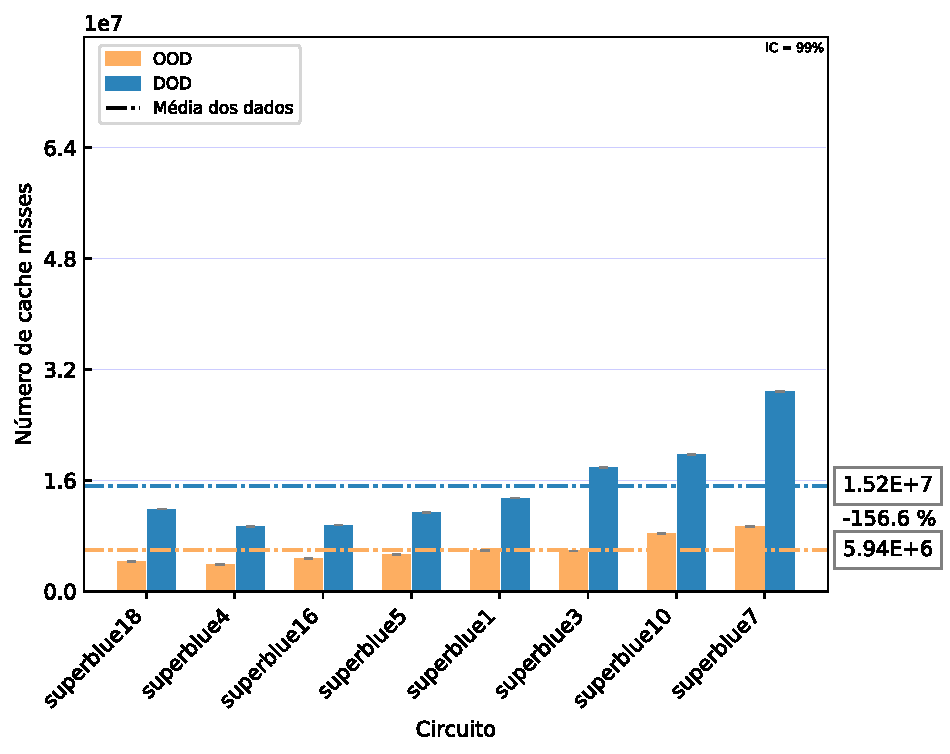
\includegraphics[width=0.47\linewidth]{img/results/problem2/problem2_miss_parallel.pdf} \label{fig:missParallelProblem2}}
    % \hspace{1cm}
    \subfigure[Tempo de execução.]{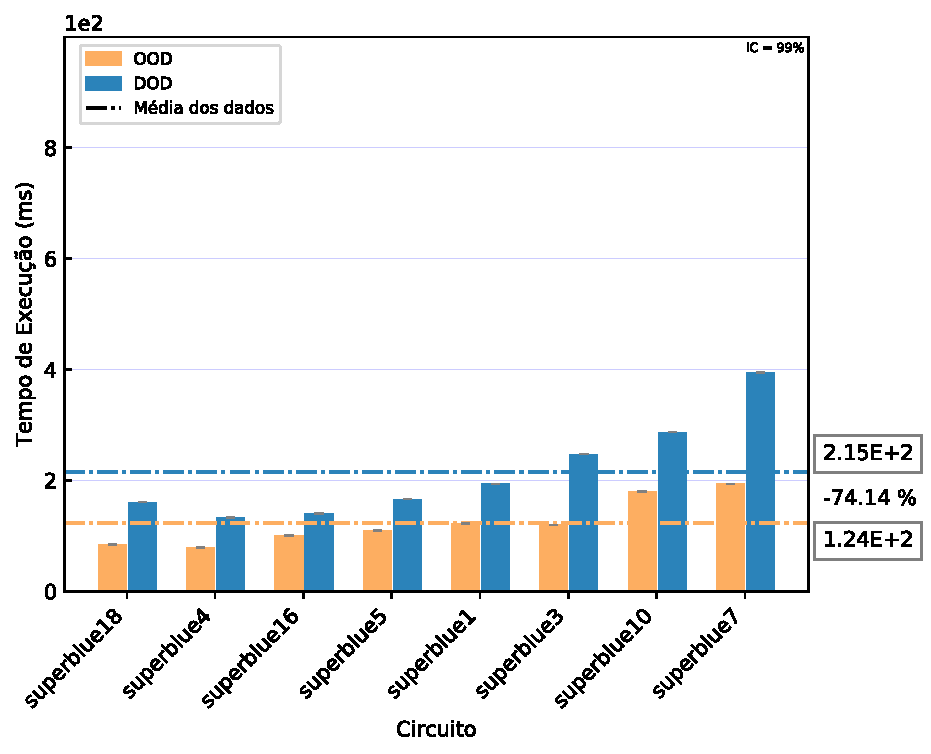
\includegraphics[width=0.47\linewidth]{img/results/problem2/problem2_runtime_parallel.pdf} \label{fig:runtimeParallelProblem2}}
    \caption[Resultados estudo de caso 2 com execução paralela]{Resultados com execução paralela.}
    \label{fig:problem2resultParallel}
\end{figure}

É possível observar que a versão paralela resultou numa redução significativa em ambas as métricas (número de  \textit{cache misses} e tempo de execução) para os dois modelos de programação. Esta redução foi mais significativa para o modelo \ac{dod}. Isto provavelmente se deve ao fato do compartilhamento de blocos recuperados da memória principal entre unidades de processamento. Contudo, mesmo com a paralelização do código, a diferença relativa entre as duas abordagens foi de $-157\%$ para o número de  \textit{cache misses} e de $-74\%$ no tempo de execução.



% \begin{figure}[ht]
%     \centering
%     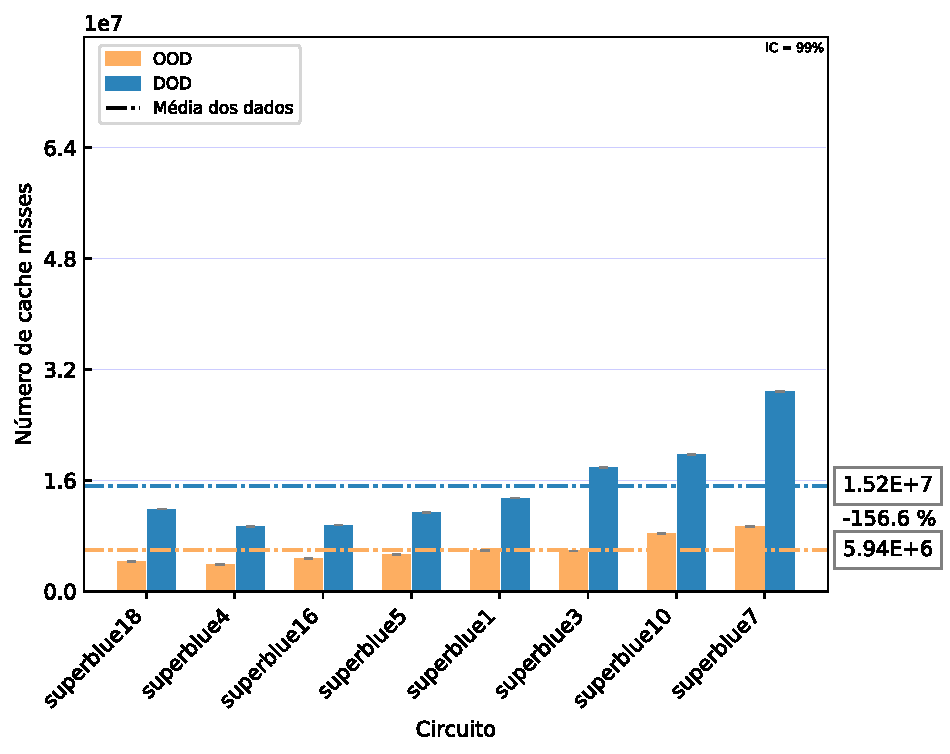
\includegraphics[width=0.65\linewidth]{img/results/problem2/problem2_miss_parallel.pdf}
%     \caption[Cache misses do Problema~2 paralelo.]{Número de cache misses resultantes dos dois protótipos de software do Problema~2 com execução paralela.}
%     \label{fig:missParallelProblem2}
% \end{figure}

% \begin{figure}[ht]
%     \centering
%     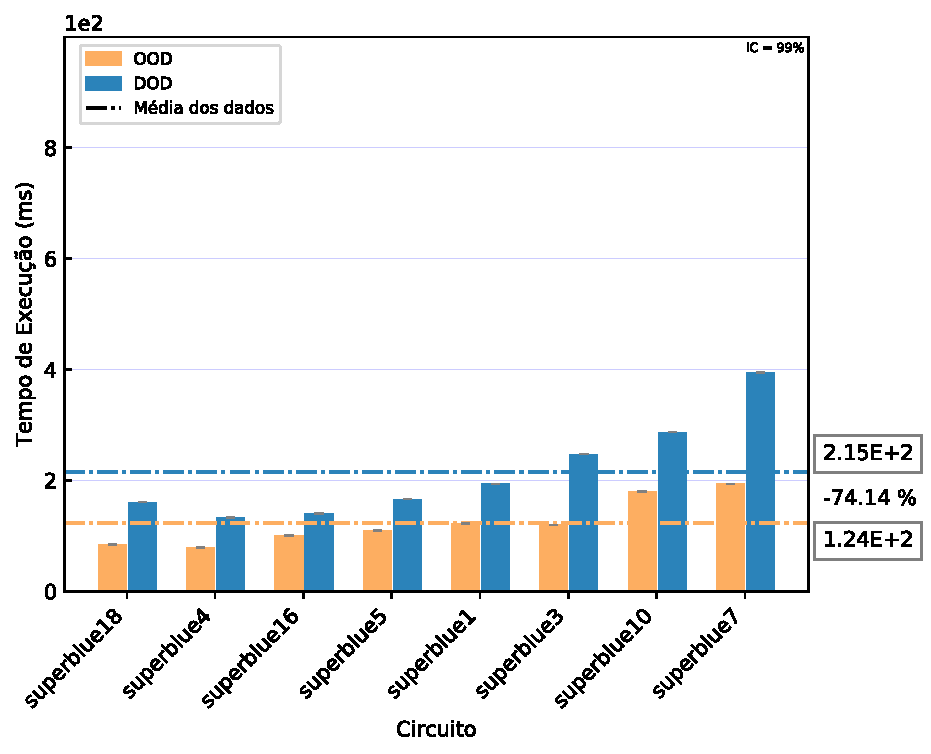
\includegraphics[width=0.65\linewidth]{img/results/problem2/problem2_runtime_parallel.pdf}
%     \caption[Tempo de execução Problema~2 paralelo]{Tempo de execução para o Problema~2 com execução paralela.}
%     \label{fig:runtimeParallelProblem2}
% \end{figure}


% AGRUPANDO AS POSIÇÕES DOS PINOS



Uma forma de melhorar a localidade espacial da posição de cada pino pertencente à mesma interconexão é agrupar esta propriedade em relação às interconexões.
Isto pode ser feito replicando os dados e aplicando, uma única vez, um algoritmo de agrupamento. 
A Figura~\ref{fig:problem2Modelagem_DOD_grouped} apresenta uma possível organização dos dados para o modelo \ac{dod} com replicação das entidades pinos e suas respectivas posições. 
Note que a única alteração da organização dos dados apresentada na Figura~\ref{subfig:problem2ModelagemDados_DOD} é a adição de dois novos vetores: \textit{Grouped Pins} e \textit{Grouped Pin Positions}.
O vetor \textit{Grouped Pins} foi agrupado com relação ao vetor \textit{Nets}, ou seja, os pinos pertencentes a cada interconexão estão armazenados de forma contígua neste vetor. Para refletir esse agrupamento, o vetor \textit{Grouped Pin Position} também segue a mesma indexação do vetor \textit{Grouped Pins}.

\begin{figure}[h!]
    \centering
    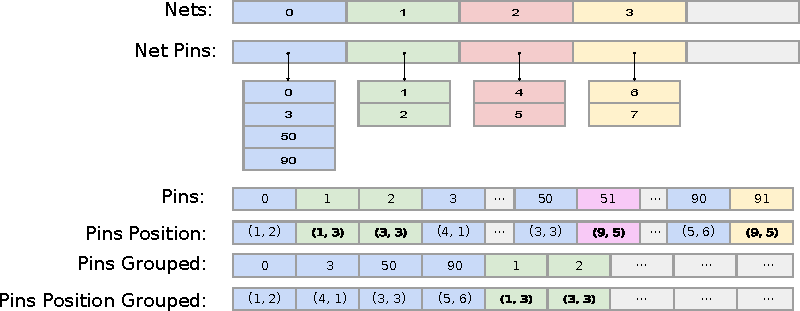
\includegraphics[width=\linewidth]{img/results/problem2/estimativa_interconection_dod_grouped.pdf}
    \caption[Agrupamento dos dados para o estudo de caso 2]{Organização dos dados para o estudo de caso 2 segundo modelo DOD. Nesta modelagem os dados referentes aos pinos foram replicados para gerar uma cópia com o agrupamento de informações.}
    \label{fig:problem2Modelagem_DOD_grouped}
\end{figure}


As Figuras~\ref{fig:problem2resultSequencialordered}~e~\ref{fig:problem2resultParallelordered} apresentam os resultados desta organização dos dados (para o modelo \ac{dod}) para execução sequencial e paralela, respectivamente. 
As barras amarelas representam o modelo de dados Orientado a Objetos (\ac{ood}), enquanto as barras azuis representam o modelo Orientado a Dados (\ac{dod}).
Os dados presentes para o modelo \ac{ood} seguem a organização apresentada na Figura~\ref{subfig:problem2ModelagemDados_OOD} da Subseção~\ref{subsec:modelagemDadosProblem2}.
Analisando os resultados para a execução sequencial, é possível observar que o número de  \textit{cache misses} reduziu, em média, duas ordens de grandeza (de $1.53\times10^7$ para $5.83\times10^5$) para o modelo \ac{dod}. Com isso, a diferença relativa entre os modelos passou a ser de $85.31\%$. Este resultado demonstra que a organização dos dados para o modelo \ac{dod} inicialmente proposta na Subseção~\ref{subsec:modelagemDadosProblem2} gerou uma baixa localidade espacial nos vetores de pinos e suas posições.
Outro benefício gerado pelo agrupamento das informações foi a vetorização do código gerado pelo compilador. Na versão proposta na Subseção~\ref{subsec:modelagemDadosProblem2} somente instruções \ac{sisd} foram traduzidas do código fonte. Porém, com a organização dos dados proposta pela Figura~\ref{fig:problem2Modelagem_DOD_grouped}, o compilador gerou instruções \ac{simd} para este estudo de caso.

\begin{figure}[ht]
    \centering
    \subfigure[Número de  \textit{cache misses}.]{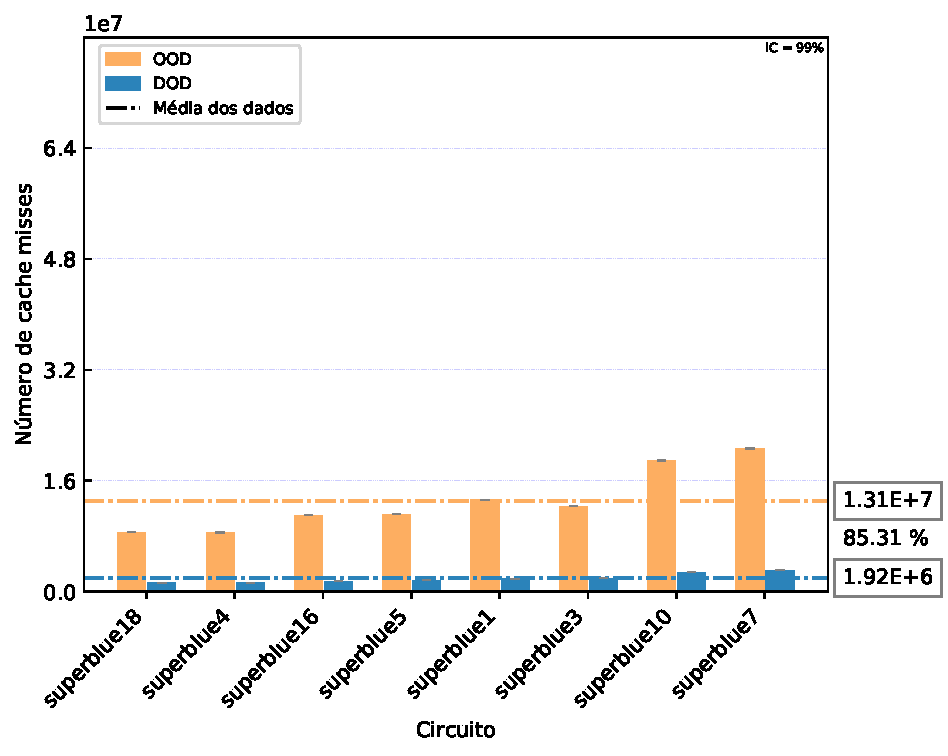
\includegraphics[width=0.47\linewidth]{img/results/problem2/problem2_miss_sequential_property_ordered.pdf} \label{fig:missSequentialProblem2ordered}}
    % \hspace{1cm}
    \subfigure[Tempo de execução.]{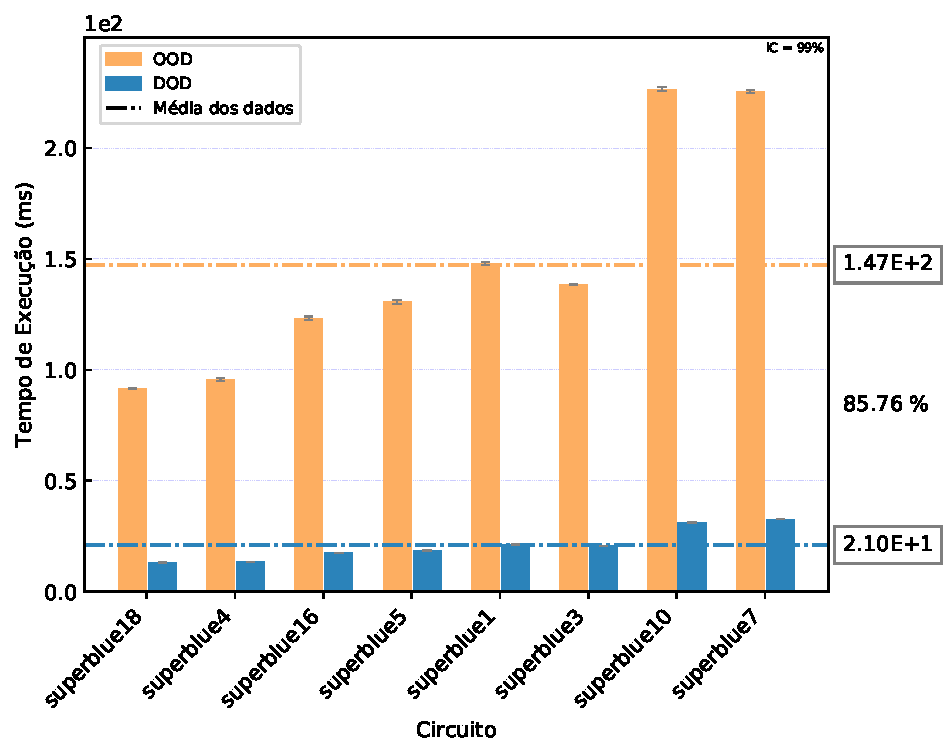
\includegraphics[width=0.47\linewidth]{img/results/problem2/problem2_runtime_sequential_property_ordered.pdf} \label{fig:runtimeSequentialProblem2ordered}}
    \caption{Resultados do estudo de caso 2 com execução sequencial e agrupamento de propriedades.}
    \label{fig:problem2resultSequencialordered}
\end{figure}

% \begin{figure}[ht]
%     \centering
%     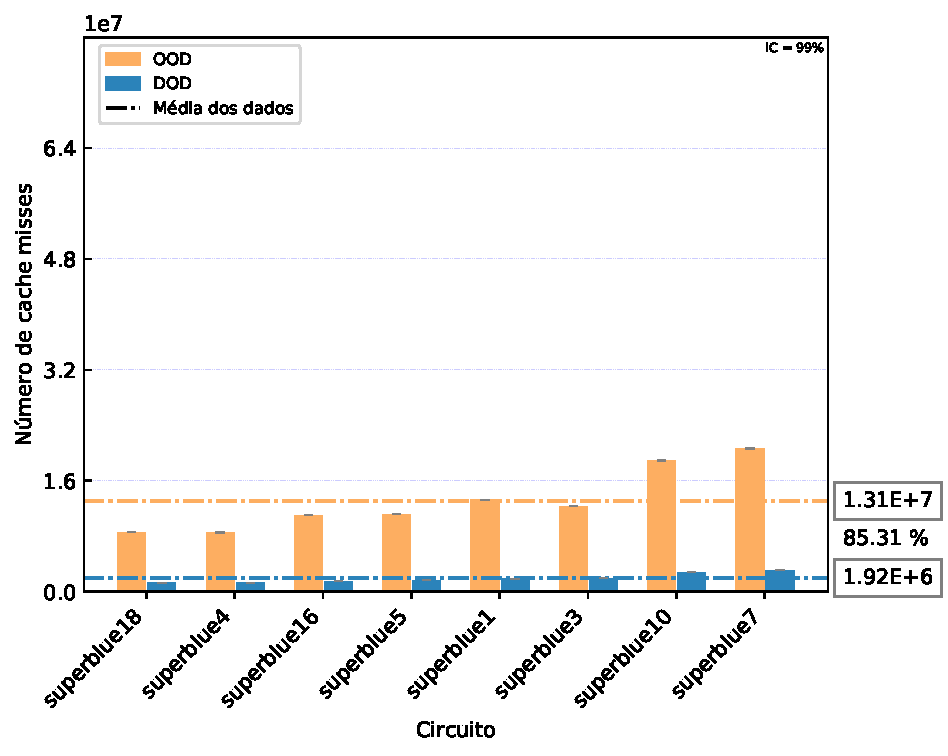
\includegraphics[width=0.65\linewidth]{img/results/problem2/problem2_miss_sequential_property_ordered.pdf}
%     \caption[Cache misses do Problema~2 sequencial com ordenamento.]{Número de cache misses resultantes dos dois protótipos de software do Problema~2 com execução sequencial.}
%     \label{fig:missSequentialProblem2ordered}
% \end{figure}

% \begin{figure}[ht]
%     \centering
%     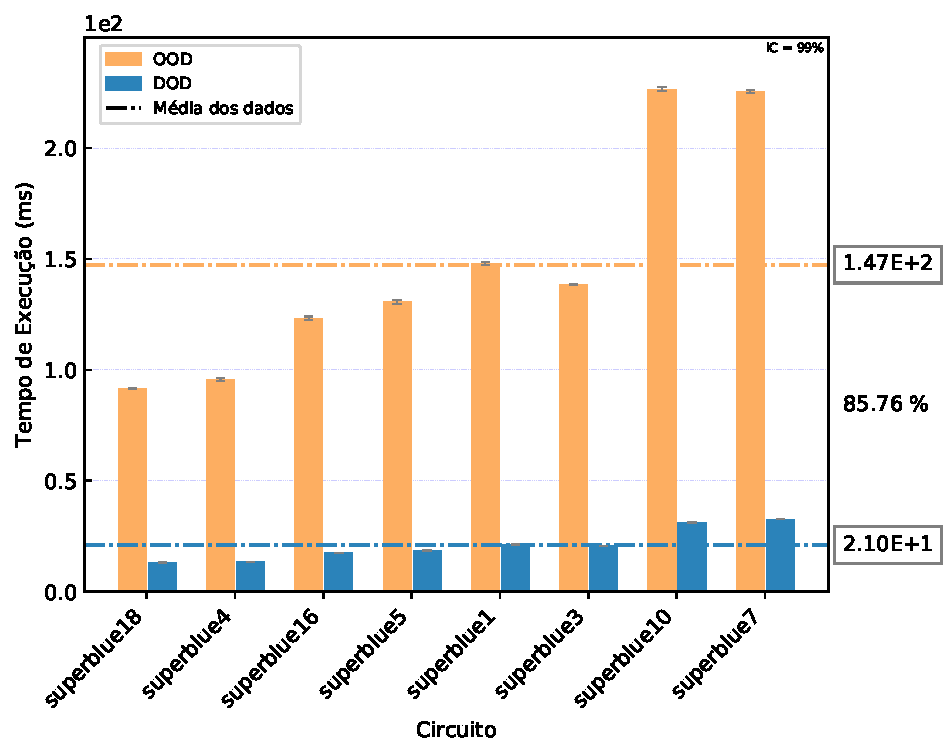
\includegraphics[width=0.65\linewidth]{img/results/problem2/problem2_runtime_sequential_property_ordered.pdf}
%     \caption[Tempo de execução Problema~2 sequencial com ordenamento.]{Tempo de execução para o Problema~2 com execução sequencial com ordenamento..}
%     \label{fig:runtimeSequentialProblem2ordered}
% \end{figure}

A Figura~\ref{fig:runtimeSequentialProblem2ordered} apresenta os resultados do tempo de execução. A escala desta figura foi alterada em relação a escala apresentada na Figura~\ref{fig:runtimeSequentialProblem2}. Esta alteração na escala fez-se necessária para ser possível visualizar os tempos de execução para o modelo \ac{dod}.
Comparando as duas execuções sequenciais, pode-se observar que o modelo \ac{dod} atingiu uma redução de uma ordem de grandeza e gerou uma diferença relativa entre as técnicas de $85\%$. 
Ou seja, o modelo \ac{dod} resulta em menos \textit{cache misses} do que \ac{ood} quando os dados estão agrupados de forma mais eficiente.
É importante observar que esse agrupamento não é possível ser feito no modelo \ac{ood} porque a posição de cada pino é armazenada internamente ao objeto \textit{Placement::Pin}.
Com isso, não é possível manter diversos agrupamentos (um para cada necessidade de algoritmos) com o modelo \ac{ood}.


Na Figura~\ref{fig:problem2resultParallelordered} são apresentados os resultados para a execução paralela do estudo de caso 2.
É possível observar que a execução paralela com dados agrupados atingiu uma taxa de redução superior àquela obtida pela paralelização sem agrupamento de informações.
Na Figura~\ref{fig:missParallelProblem2ordered} é apresentado o número de  \textit{cache misses} (eixo Y) para cada circuito avaliado (eixo X).
O modelo \ac{ood} gerou entre $3M$ e $9M$ de \textit{cache misses}, tendo em média $5$ milhões de  \textit{cache misses} para cada circuito.
Já o modelo \ac{dod} gerou entre $374k$ e $1M$ de \textit{cache misses}, tendo em média $583$ mil  \textit{cache misses} para cada circuito. 
A diferença relativa entre os dois modelos foi, em média, de $90\%$.

Na Figura~\ref{fig:runtimeParallelProblem2ordered} estão apresentados os tempos de execução da execução paralela (eixo Y) em milissegundos para cada circuito avaliado (eixo X).
Os tempos de execução foram de $78ms$ a $193ms$ para o modelo \ac{ood} e de $4ms$ a $10ms$ para o modelo \ac{dod}.





\begin{figure}[ht]
    \centering
    \subfigure[Número de  \textit{cache misses}.]{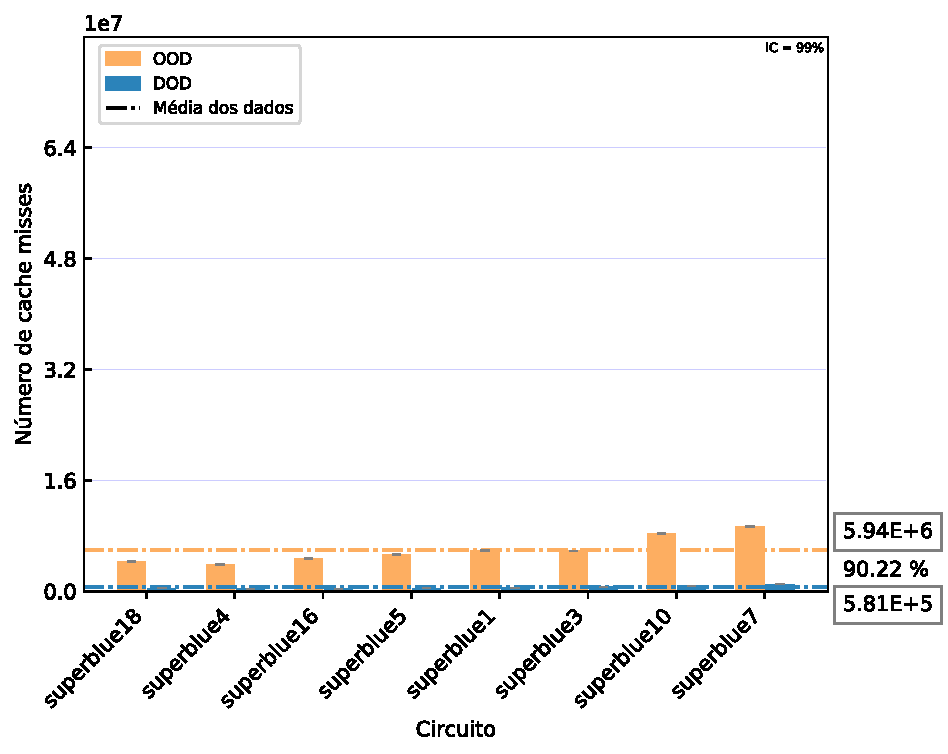
\includegraphics[width=0.47\linewidth]{img/results/problem2/problem2_miss_parallel_property_ordered.pdf} \label{fig:missParallelProblem2ordered}}
    % \hspace{1cm}
    \subfigure[Tempo de execução.]{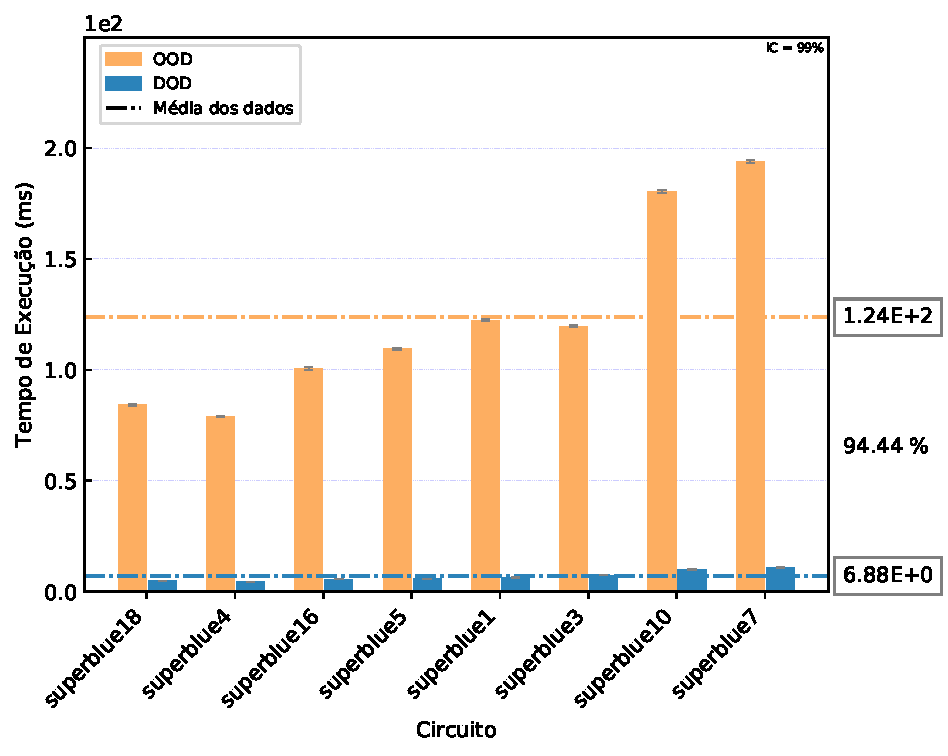
\includegraphics[width=0.47\linewidth]{img/results/problem2/problem2_runtime_parallel_property_ordered.pdf} \label{fig:runtimeParallelProblem2ordered}}
    \caption{Resultados do estudo de caso 2 com execução paralela e agrupamento de propriedades.}
    \label{fig:problem2resultParallelordered}
\end{figure}

% \begin{figure}[ht]
%     \centering
%     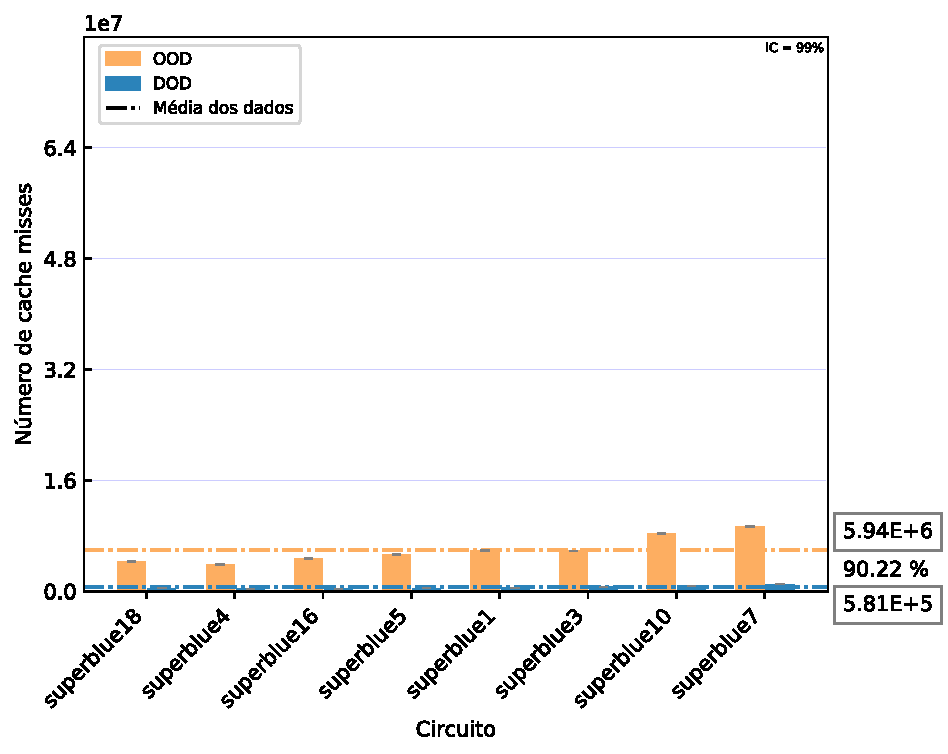
\includegraphics[width=0.65\linewidth]{img/results/problem2/problem2_miss_parallel_property_ordered.pdf}
%     \caption[Cache misses do Problema~2 paralelo com ordenamento..]{Número de cache misses resultantes dos dois protótipos de software do Problema~2 com execução paralela com ordenamento.}
%     \label{fig:missParallelProblem2ordered}
% \end{figure}

% \begin{figure}[ht]
%     \centering
%     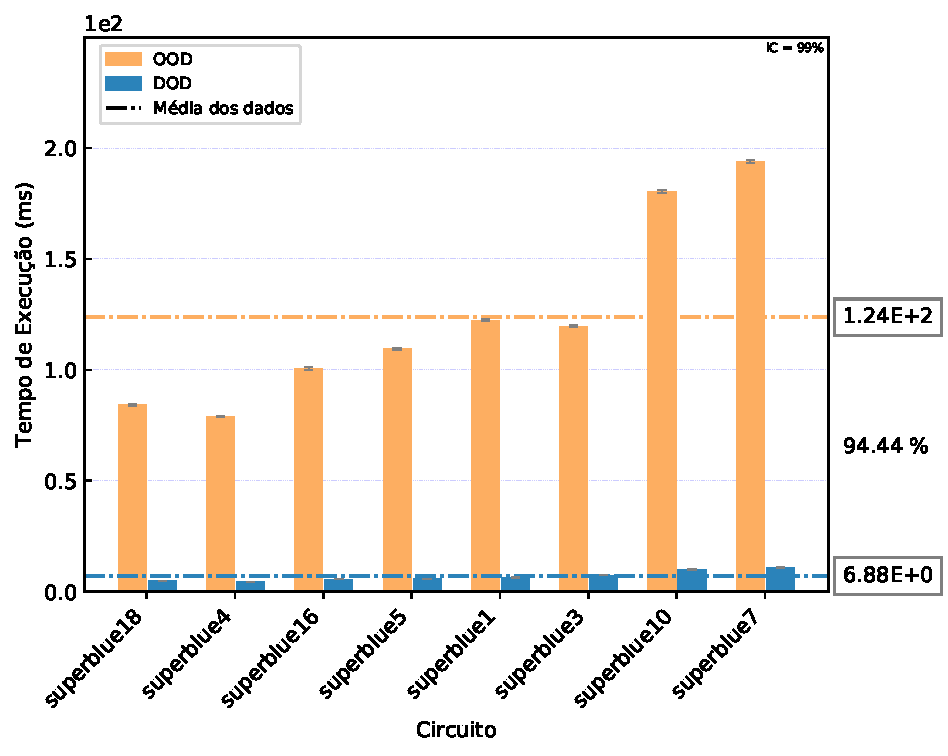
\includegraphics[width=0.65\linewidth]{img/results/problem2/problem2_runtime_parallel_property_ordered.pdf}
%     \caption[Tempo de execução Problema~2 paralelo com ordenamento.]{Tempo de execução para o Problema~2 com execução paralela com ordenamento.}
%     \label{fig:runtimeParallelProblem2ordered}
% \end{figure}




\section{Estudo de caso 3: Clusterização de Registradores}
\label{sec:estudo_de_caso_3}

Este estudo de caso avalia uma tarefa com maior intensidade aritmética e com poucas propriedades.
Durante a etapa de \textit{Clock Tree Synthesis} os registradores próximos são agrupados para que um \textit{buffer} do sinal de relógio possa ser inserido. Este processo é denominado clusterização dos registradores. Dado um conjunto de posições dos registradores $\mathcal{R} = \{r_1, r_2, ..., r_n\}$ onde cada $r_i \in \mathbb{R}^2$, o problema de clusterizar os registradores pode ser definido como: particionar o conjunto $\mathcal{R}$ num número predefinido $k$ de \textit{clusters} $\Gamma = \{\gamma_1, \gamma_2, ..., \gamma_k\}$ onde a soma das interconexões pertencentes a cada \textit{cluster} seja minimizada. A soma das interconexões está descrita pelas Equações \eqref{eq:register_clustering} a \eqref{eq:union_constraint}.
Cada $\gamma_i \in \Gamma$ representa o conjunto de elementos pertencentes ao \textit{cluster} $i$.
A Equação~\eqref{eq:register_clustering} apresenta a função objetivo definida pela soma das distâncias Manhattan entre o centro de cluster $c_i$ e os elementos pertencentes a este cluster.
Geralmente, o centro do cluster é determinado pelo centro gravitacional de seus elementos: $c_i = \sum_{r_j \in \gamma_i} r_j/|\gamma_i|$, onde $|\gamma_i|$ representa o tamanho  de $\gamma_i$.
As Equações \eqref{eq:empty_constraint} a \eqref{eq:union_constraint} definem as partições de $\mathcal{R}$, isto é, cada registrador deve pertencer a um, e somente um \textit{cluster}.

\simbolo{$\mathcal{R}$}{conjunto de registradores $\mathcal{R}$ do circuito}
\simbolo{$\Gamma$}{conjunto de \textit{clusters} do circuito}
\simbolo{$\gamma_i$}{i-ésimo \textit{clister} do conjunto $\Gamma$}

\begin{eqnarray}
\label{eq:register_clustering}
    \textbf{Min}&:& \sum_{i = 1}^{k}\sum_{r_j \in \gamma_i} \lVert c_i - r_j\rVert_2^2 \\
    % \label{eq:cluster_mean}
    % && x_{cl_i} = \frac{\sum_{r_j \in cl_i} x_{r_j}}{|cl_i|}, \ y_{cl_i} = \frac{\sum_{r_j \in cl_i} y_{r_j}}{|cl_i|} \\
    \label{eq:empty_constraint}
    \textbf{S.t.} &:& \gamma_i \in \Gamma \implies \gamma_i \neq \emptyset \\
    \label{eq:intersection_constraint}
    &:&\gamma_i, \gamma_j \in \Gamma \ \land \ i \neq j \implies \gamma_i \cap \gamma_j = \emptyset\\
    \label{eq:union_constraint}
    &:& \mathcal{R} = \bigcup_{\gamma_i \in \Gamma} \gamma_i 
\end{eqnarray}

Um algoritmo clássico de clusterização de elementos é o \textit{K-means} \cite{selim1984k}.
Este algoritmo não é somente utilizado para clusterização de registradores, mas também em diferentes áreas como \textit{machine learning} e \textit{data mining}.
O Algoritmo~\ref{alg:problem3} descreve as etapas do \textit{k-means}.
Este algoritmo recebe como entrada um conjunto $\mathcal{R}$ de posições de registradores e um conjunto $\mathcal{C}$ dos $k$ centros de \textit{clusters}.
Existem diversas formas de determinar o número $k$ de \textit{clusters}. Neste trabalho o número máximo de elementos por \textit{cluster} foi limitado a $50$.
Portanto, o número $k$ de cluster para cada circuito foi determinado pelo número de registradores dividido por $50$ ($k=\lceil\frac{|\mathcal{R}|}{50}\rceil$).
A posição de cada centro de \textit{cluster} foi inicializada aleatoriamente com uma distribuição uniforme.
O retorno do algoritmo é um conjunto de \textit{clusters} e seus novos centros.

\begin{algorithm}[bht]
\SetKwInOut{Input}{Entrada}\SetKwInOut{Output}{Saída}
\SetKwRepeat{Do}{do}{while}
\LinesNumbered
     \Input{Conjunto $\mathcal{R}$ de posições dos registradores, conjunto $\mathcal{C}$ dos $k$ centros de clusters} 
     \Output{Conjunto de clusters $\Gamma$ e seus respectivos centros $\mathcal{C}$}
     \Do{centros dos clusters não convergirem}{
        $\gamma_i \gets \emptyset, \ i = 1 \dots k$\; \label{line:clear}
        \ForEach{$r_i \in \mathcal{R}$}{ \label{line:for_assignment_init}
            $c_j \gets \argmin_{c_j \in \mathcal{C}} \{\lVert c_j - r_i\rVert_2^2  \}$\; \label{alg:problem3:buscaRTree}
            $\gamma_j \gets \gamma_j \cup \{r_i\}$\;
        } \label{line:for_assignment_end}
        % $\Gamma \gets \bigcup_{i = 1}^k \gamma_i$\;
        \ForEach{$\gamma_i \in \Gamma$}{
            $c_i \gets \sum_{r_j \in \gamma_i} r_j/|\gamma_i|$\;
        }
     }
  \caption{\textit{K-means}} \label{alg:problem3}
\end{algorithm}

Inicialmente todos os \textit{clusters} estão vazios (line~\ref{line:clear}).
Então, o algoritmo resolve o problema da clusterização de registradores executando duas etapas principais: \textbf{assinalamento} e \textbf{atualização}.
Durante a etapa de assinalamento (linhas 3 a 6), cada registrador é assinalado para o centro de \textit{cluster} mais próximo da  sua posição.
Após assinalar todos os registradores para um cluster, na etapa de atualização (linhas 7 a 9), os centros dos \textit{clusters} são realocados para o centro de massa de seus elementos.
Estas duas etapas são executadas até que todos os centros dos \textit{clusters} convirjam ou um número máximo de iterações seja atingido.
Neste trabalho o número de iterações foi limitado a 10 e utilizou-se a mesma semente na geração das posições iniciais aleatórias dos centros dos \textit{clusters}.

% \begin{figure}[ht]
%     \centering
%     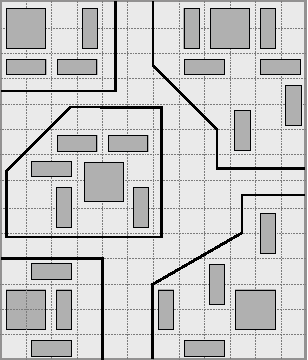
\includegraphics[width=0.3\linewidth]{img/results/problem3/problem3.pdf}
%     \caption[]{}
%     \label{fig:problem3}
% \end{figure}


\subsection{Modelagem dos Dados}
\label{subsec:modelagemDadosProblem3}
A Figura~\ref{fig:problem3ModelagemDados} apresenta uma possível modelagem dos dados para este estudo de caso.
A Figura~\ref{subfig:problem3ModelagemDados_OOD} ilustra o diagrama de classes para o modelo \ac{ood}.
Neste modelo são definidas duas classes: \textit{cluster} e \textit{Register}.
A seta com ponta de losango entre estas classes representa  uma relação de agregação --- o que significa que \textit{Cluster} possui referência para seus registradores.
Na Figura~\ref{subfig:problem3ModelagemDados_DOD} é possível observar a organização dos dados para o modelo \ac{dod}.
A agregação representada pela seta com ponta de losango entre estas classes no modelo \ac{ood} é, neste caso, realizada pelo vetor \textit{Cluster Registers}.
Também é possível observar que nesta abordagem não existem dados desnecessários (como o nome de um registrador) para o presente estudo de caso.

\begin{figure}[ht]
    \centering
    % Diagrama de classes para modelar a clusterização de registradores segundo paradigma de programação \ac{ood}.
    \subfigure[]{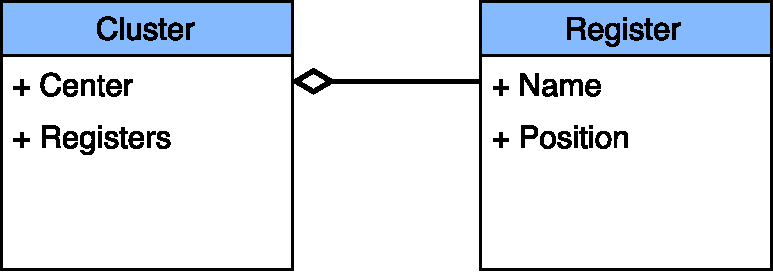
\includegraphics[width=0.35\linewidth]{img/results/problem3/problem3_OOD.pdf} \label{subfig:problem3ModelagemDados_OOD}}
    \hspace{0.1cm}
    % Modelagem dos dados para o problema de clusterizar os registradores segundo paradigma de programação \ac{dod}.
    \subfigure[]{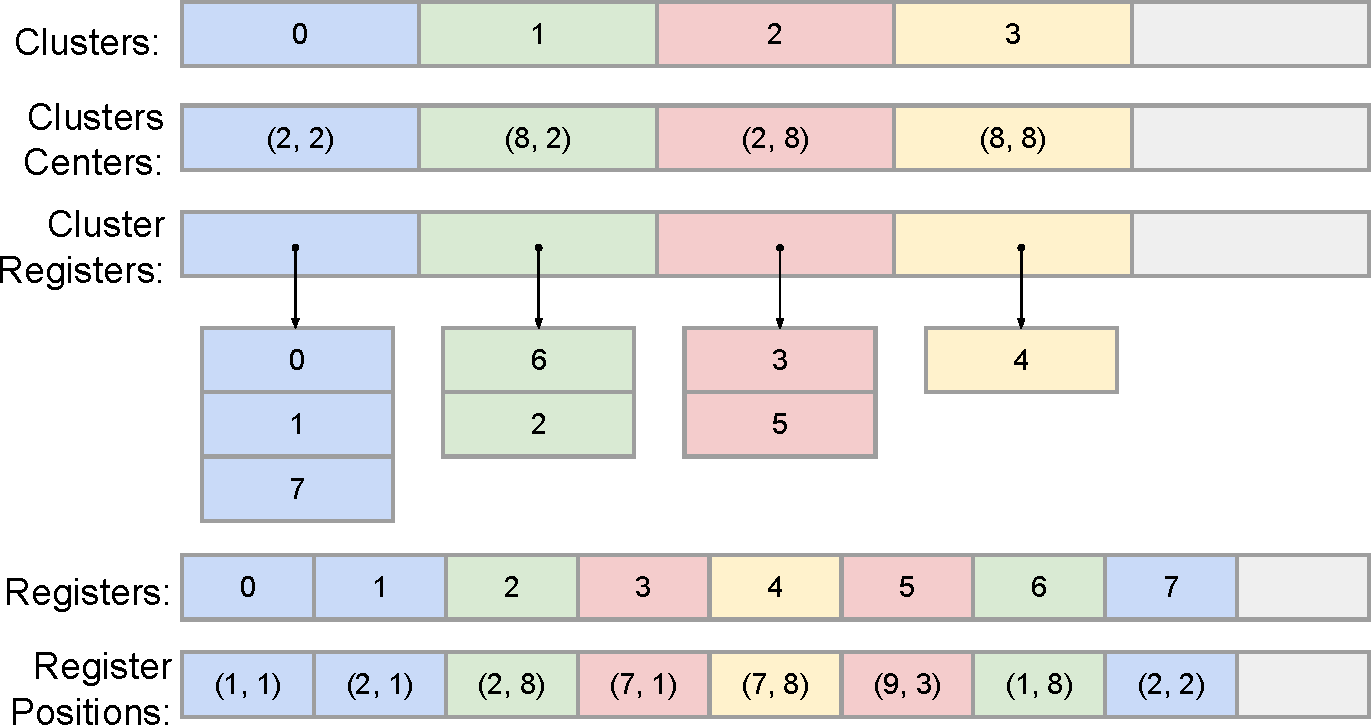
\includegraphics[width=0.55\linewidth]{img/results/problem3/problem3_DOD.pdf} \label{subfig:problem3ModelagemDados_DOD}}
    \caption[Organização dos dados estudo de caso 3]{Organização dos dados para estimativa do comprimento das interconexões segundo os modelos de programação OOD (a) e DOD (b).}
    \label{fig:problem3ModelagemDados}
\end{figure}


\subsection{Avaliação}

A Figura~\ref{fig:resultsProblem3sequential} apresenta os resultados da execução sequencial do estudo de caso 3 utilizando a modelagem dos dados descrita na Seção~\ref{subsec:modelagemDadosProblem3}. 
As barras amarelas representam o modelo de dados Orientado a Objetos (\ac{ood}), enquanto, as barras azuis representam o modelo Orientado a Dados (\ac{dod}).
Na esquerda, Figura~\ref{fig:missSequentialProblem3}, o número de  \textit{cache misses} (eixo Y) para cada circuito avaliado (eixo X). Para cada circuito, a entrada constituiu-se das posições de todos os registradores do circuito.
É possível observar que ambos os modelos (\ac{ood} e \ac{dod}) resultaram em um número muito similar de \textit{cache misses} para carregarem os dados para este estudo de caso.
Portanto, não é possível inferir informações estatísticas sobre os circuitos \textit{superblue4}, \textit{superblue5} e \textit{superblue1}, pois nestes casos há uma intersecção no intervalo de confiança entre os dois modelos. Nos demais circuitos o modelo \ac{dod} obteve um desempenho ligeiramente melhor do que o modelo \ac{ood}.
A Figura~\ref{fig:runtimeSequentialProblem3} apresenta o tempo de execução em segundos (eixo Y) para cada circuito avaliado (eixo X).
Novamente, pode-se observar que existem intersecções nos intervalos de confiança.
Portanto, não é possível estimar qual dos dois modelos obteve um melhor desempenho.

\begin{figure}[hbt]
    \centering
    \subfigure[Número de  \textit{cache misses}.]{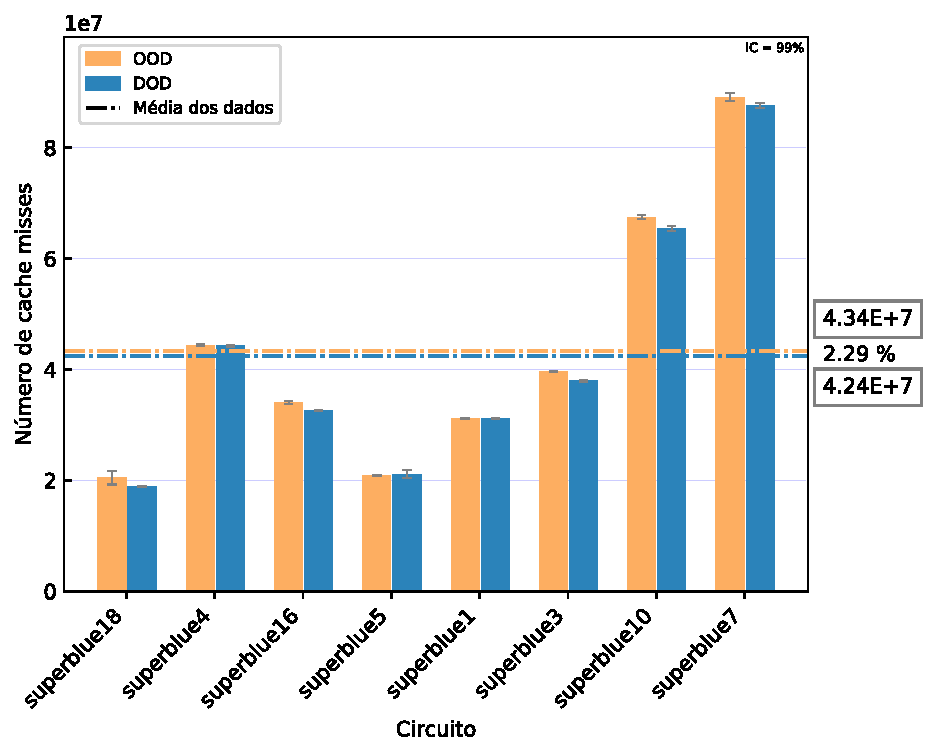
\includegraphics[width=0.47\linewidth]{img/results/problem3/problem3_miss_sequential.pdf} \label{fig:missSequentialProblem3}}
    \subfigure[Tempo de execução.]{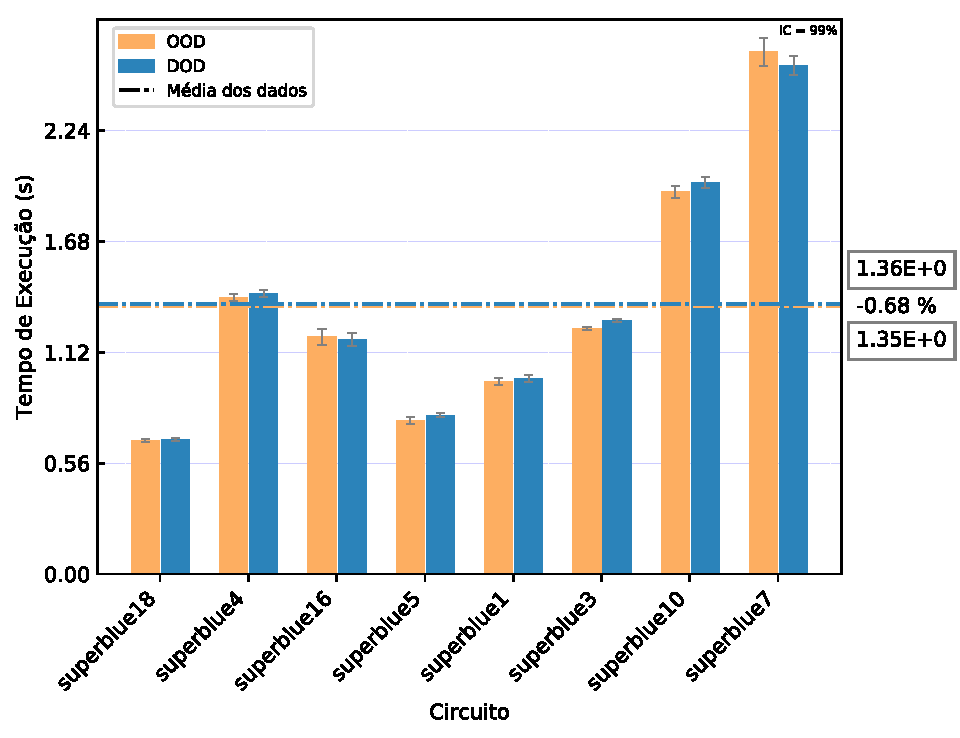
\includegraphics[width=0.47\linewidth]{img/results/problem3/problem3_runtime_sequential.pdf} \label{fig:runtimeSequentialProblem3}}
    \caption{Resultados para a execução sequencial do estudo de caso 3.}
    \label{fig:resultsProblem3sequential}
\end{figure}

Uma possível explicação para o comportamento similar entre os dois modelos é o fato de que a busca espacial pelo centro do \textit{cluster} mais próximo a cada registrador foi realizada utilizando a estrutura de dados \textit{R-Tree}~\footnote{A estrutura de dados R-tree consiste em uma árvore espacial especializada no armazenamento de dados multidimensionais.}~\cite{manolopoulos2010r} para ambos os modelos (linha~\ref{alg:problem3:buscaRTree} do Algoritmo~\ref{alg:problem3}). 
% O modelo \ac{dod} foi incapaz de atingir um alto desempenho na localidade espacial dos dados fornecidos a R-tree pois a alta intensidade aritmética esta concentrada exatamente na etapa de busca espacial e o acesso ao vetor das posições dos registradores não é garantidamente contíguo.
% Uma abordagem seria aplicar um agrupamento nas posições dos registradores pertencentes ao mesmo cluster. Isso daria garantias a localidade espacial dos dados na busca espacial.
% Porém, como um determinado registrador pode ser trocado de um \textit{cluster} para outro em cada iteração do algoritmo, seria necessário reagrupar o vetor de posições de registradores a cada iteração do algoritmo. Este sobrecusto de agrupar o vetor possivelmente é maior do que o custo gerado sem nenhum agrupamento/ordenamento dos dados.
O modelo \ac{dod} foi incapaz de atingir um alto desempenho pois a maior complexidade do algoritmo \textit{K-means} reside na busca espacial pelos \textit{clusters} próximos, realizada pela \textit{R-tree}, cuja estrutura interna independe da organização dos dados.

% \begin{figure}[ht]
%     \centering
%     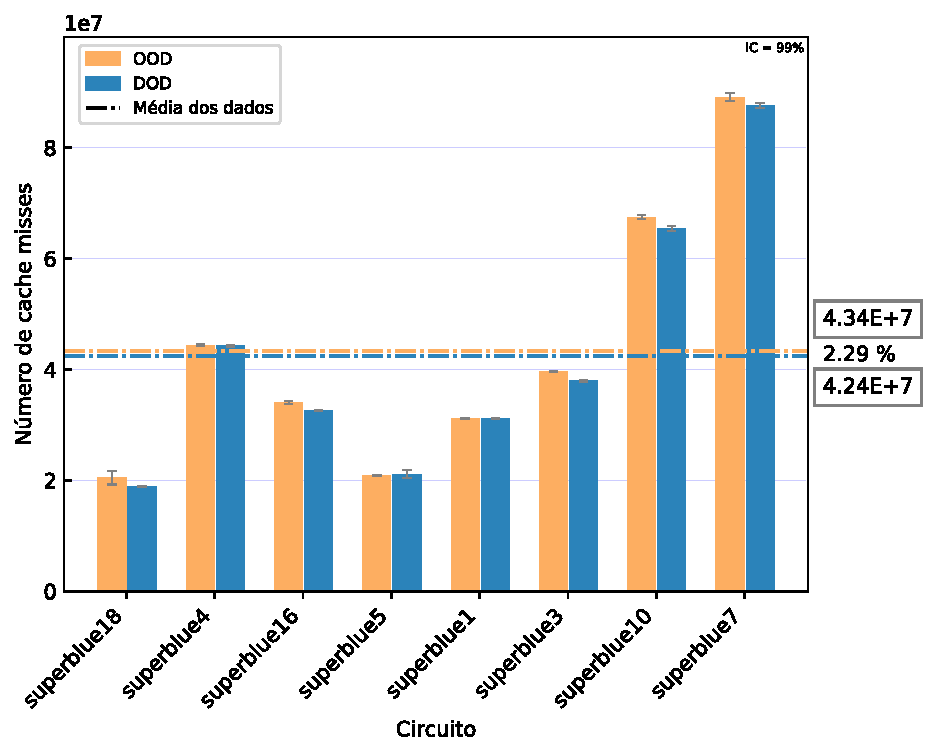
\includegraphics[width=0.65\linewidth]{img/results/problem3/problem3_miss_sequential.pdf}
%     \caption[Cache misses do Problema~3 sequencial.]{Número de cache misses resultantes dos dois protótipos de software do Problema~3 com execução sequencial.}
%     \label{fig:missSequentialProblem3}
% \end{figure}

% \begin{figure}[ht]
%     \centering
%     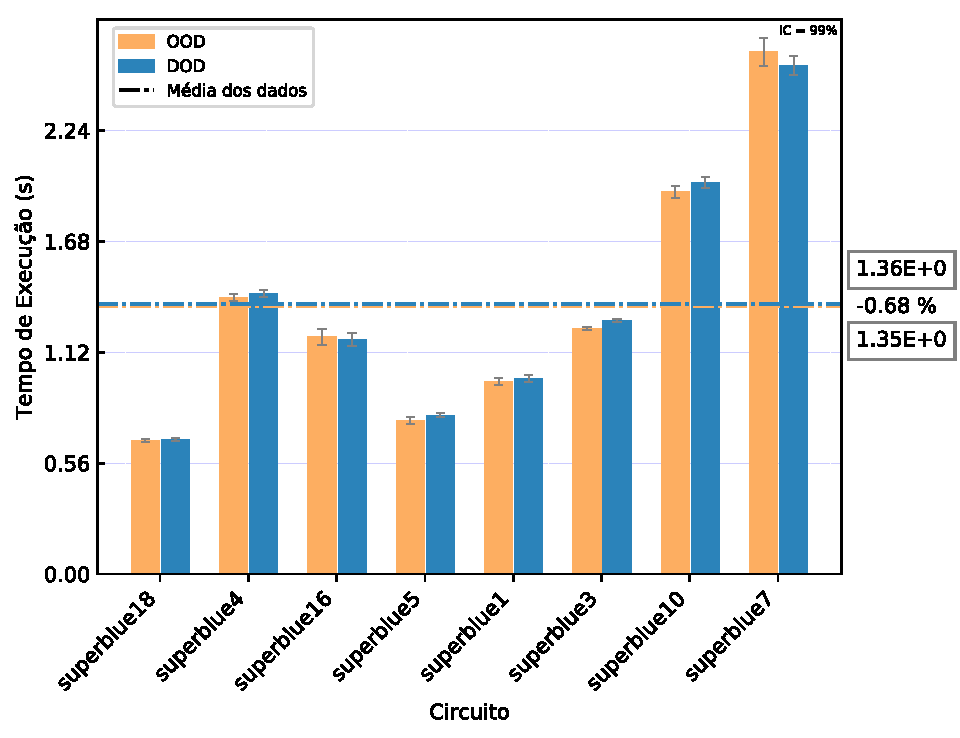
\includegraphics[width=0.65\linewidth]{img/results/problem3/problem3_runtime_sequential.pdf}
%     \caption[Tempo de execução Problema~3 sequencial]{Tempo de execução para o Problema~3 com execução sequencial.}
%     \label{fig:runtimeSequentialProblem3}
% \end{figure}

O Algoritmo~\ref{alg:problem3parallel} apresenta uma versão paralela para o Algoritmo~\ref{alg:problem3}.
Ao paralelizar a etapa de assinalamento, linhas 4 a 6 do Algoritmo~\ref{alg:problem3}, é obrigatória a adição de um mapeamento extra para o conjunto de registradores pertencentes a cada \textit{cluster} (linha 5 do Algoritmo~\ref{alg:problem3}). Isto se faz necessário pois dois registradores podem escrever simultaneamente no mesmo \textit{cluster}.
Este mapeamento é realizado com um vetor auxiliar $\alpha$ de tamanho igual ao número de registradores do circuito --- $|\alpha| = |\mathcal{R}|$.
Então, na linha 5 do Algoritmo~\ref{alg:problem3parallel}, cada registrador irá escrever numa posição única do vetor $\alpha$, retirando assim a concorrência no acesso aos \textit{clusters}.
Com este mapeamento extra, é necessário adicionar um laço para atualizar as referências dos registradores pertencentes a um \textit{cluster}.
Isto é realizado entre as linhas 7 e 10 do Algoritmo~\ref{alg:problem3parallel}.
Ao paralelizar a etapa de atualização dos \textit{clusters}, linhas  7 a 9 do Algoritmo~\ref{alg:problem3}, não se faz necessária nenhuma alteração no código fonte, uma vez que cada cluster irá escrever em variáveis distintas.

\begin{algorithm}[h!t]
\SetKwInOut{Input}{Entrada}\SetKwInOut{Output}{Saída}
\SetKwRepeat{Do}{do}{while}
\LinesNumbered
     \Input{Conjunto $\mathcal{R}$ de posições dos registradores, conjunto $\mathcal{C}$ dos $k$ centros de clusters} 
     \Output{Conjunto de clusters $\Gamma$ e seus respectivos centros $\mathcal{C}$}
     \Do{centros dos clusters não convergirem}{
        $\gamma_i \gets \emptyset, \ i = 1 \dots k$\;
        % $\alpha \gets \emptyset, \ i = 1 \dots k$\;
        \textit{\textbf{\#pragma omp parallel for}} \hspace{75pt} \ForEach{$r_i \in \mathcal{R}$}{
            $c_j \gets \argmin_{c_j \in \mathcal{C}}\{\lVert c_j - r_i\rVert_2^2 \}$\;
            $\alpha_i \gets \gamma_j$\;
        }
        
        \ForEach{$r_i \in \mathcal{R}$}{        
            $\gamma_j \gets \alpha_i$\;
            $\gamma_j \gets \gamma_j \cup \{r_i\}$\;
        }
        
        % $\Gamma \gets \bigcup_{i = 1}^k \gamma_i$\;
        \textit{\textbf{\#pragma omp parallel for}} \hspace{75pt} \ForEach{$\gamma_i \in \Gamma$}{
            $c_i \gets \sum_{r_j \in \gamma_i} r_j/|\gamma_i|$\;
        }
     }
  \caption{\textit{K-means} em paralelo}
  \label{alg:problem3parallel}
\end{algorithm}



\begin{figure}[h!b]
    \centering
    \subfigure[Número de  \textit{cache misses}.]{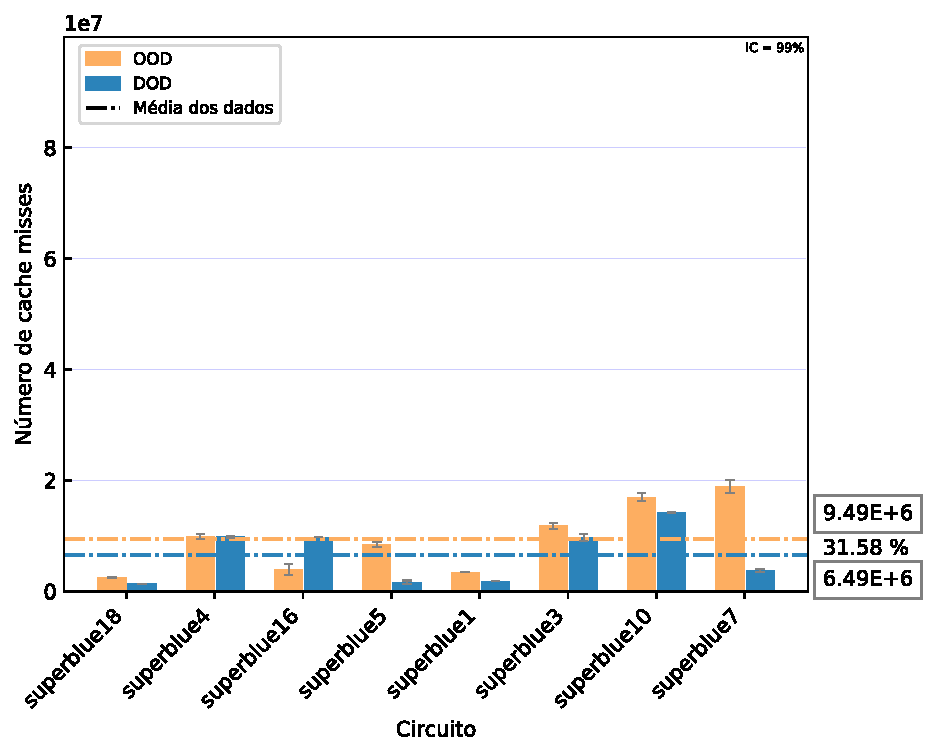
\includegraphics[width=0.47\linewidth]{img/results/problem3/problem3_miss_parallel.pdf} \label{fig:missParallelProblem3}}
    \subfigure[Tempo de execução.]{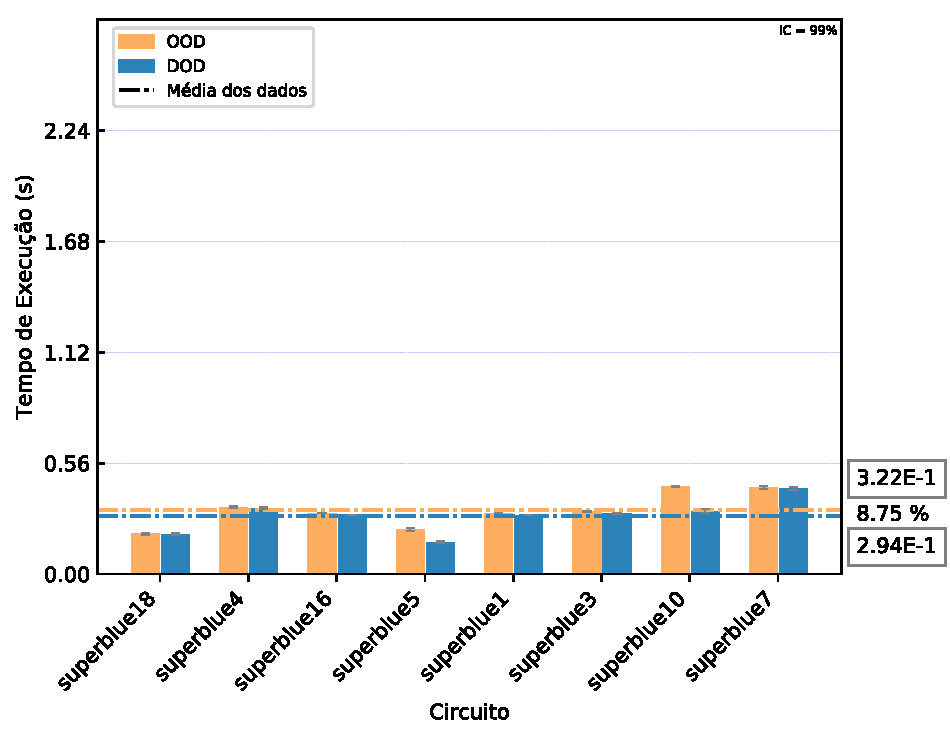
\includegraphics[width=0.47\linewidth]{img/results/problem3/problem3_runtime_parallel.pdf} \label{fig:runtimeParallelProblem3}}
    \caption{Resultados para a execução paralela do estudo de caso 3.}
    \label{fig:resultsProblem3parallel}
\end{figure}

A Figura~\ref{fig:resultsProblem3parallel} apresenta os resultados da execução paralela do estudo de caso 3.
As barras amarelas representam o modelo de dados Orientado a Objetos (\ac{ood}), ao passo que as barras azuis representam o modelo Orientado a Dados (\ac{dod}).
É possível observar que, ao paralelizar o algoritmo k-means, o modelo \ac{dod} favoreceu a localidade espacial e reduziu o número de  \textit{cache misses} para a maioria dos circuitos.
O número de  \textit{cache misses} para o modelo \ac{ood} foi em média $9.49M$, com coeficiente de variação\footnote{O coeficiente de variação $cv$ é definido como $cv = \frac{\sigma}{\mu}$ onde $\sigma$ e $\mu$ representam respectivamente o desvio padrão e a média.} médio de $13\%$.
Para o modelo \ac{dod}, o número de  \textit{cache misses} foi, em média, $6.49M$, e teve um coeficiente de variação de $10\%$.



% \begin{figure}[ht]
%     \centering
%     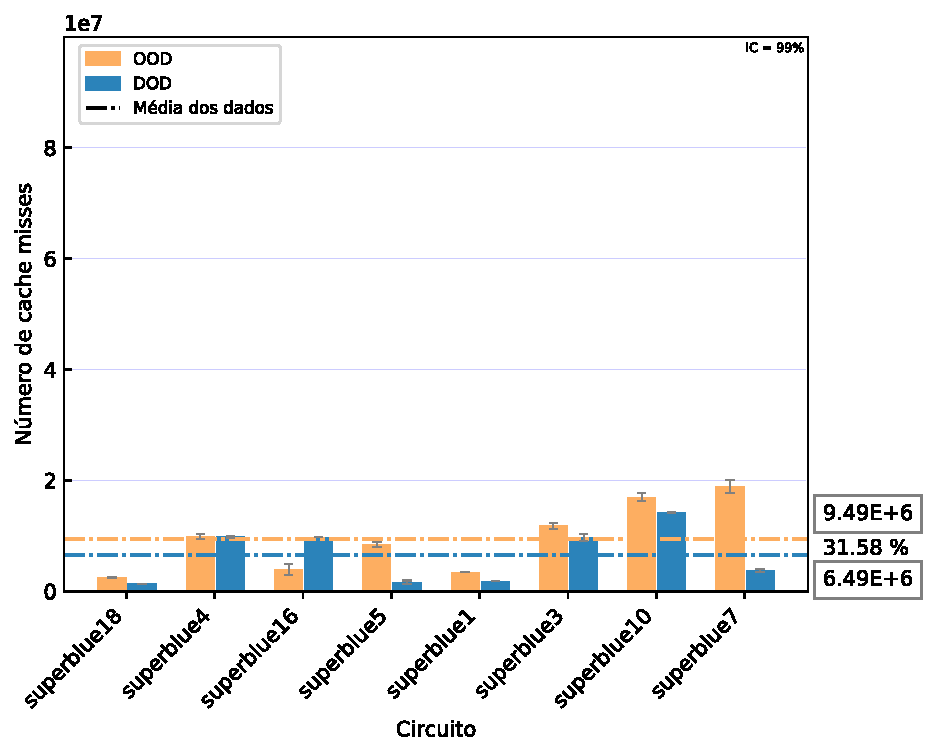
\includegraphics[width=0.65\linewidth]{img/results/problem3/problem3_miss_parallel.pdf}
%     \caption[Cache misses do Problema~3 paralelo.]{Número de cache misses resultantes dos dois protótipos de software do Problema~3 com execução paralela.}
%     \label{fig:missParallelProblem3}
% \end{figure}

% \begin{figure}[ht]
%     \centering
%     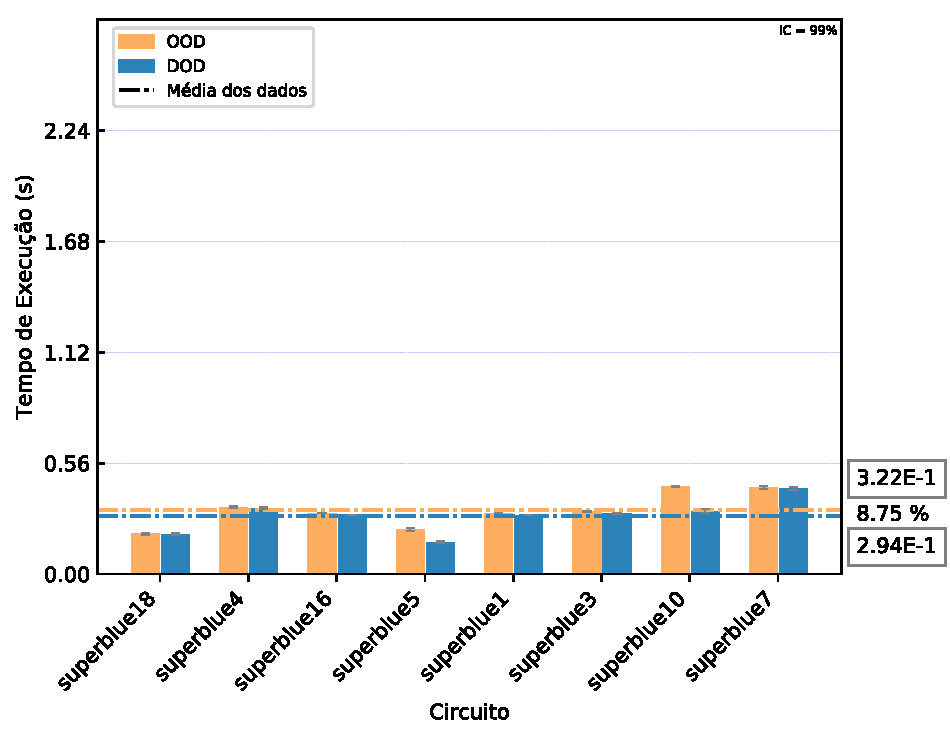
\includegraphics[width=0.65\linewidth]{img/results/problem3/problem3_runtime_parallel.pdf}
%     \caption[Tempo de execução Problema~3 paralelo]{Tempo de execução para o Problema~3 com execução paralela.}
%     \label{fig:runtimeParallelProblem3}
% \end{figure}

A Figura~\ref{fig:runtimeParallelProblem3} apresenta os tempos de execução (eixo Y), em segundos, para cada circuito avaliado (eixo X).
O modelo \ac{dod} foi mais rápido que o modelo \ac{ood} em todos os circuitos avaliados.
O modelo \ac{ood} executou entre $0.20$ (no circuito \textit{superblue18}) e $0.44$ (no circuito \textit{superblue10}) segundos. Em média, este modelo levou $0.32$ segundos com desvio padrão médio de $2.77\%$ em relação à média das execuções. 
Já o modelo \ac{dod} executou entre $0.16$ (no circuito \textit{superblue5}) e $0.43$ (no circuito \textit{superblue7}) segundos, com média de $0.29$ segundos e desvio padrão médio de $3.28\%$ em relação a média das execuções.
A diferença relativa entre as duas técnicas foi de $8.75\%$, o que sugere que a implementação \ac{dod} apresenta maior potencial de paralelismo neste problema.




\section{Estudo de caso 4: Roteamento global}
\label{sec:estudo_de_caso_4}

Este estudo de caso avalia tarefas que possuem suas informações representadas por meio de um grafo.
Durante a etapa de síntese física de um \ac{ic}, a etapa de roteamento global é responsável por interconectar os pinos pertencentes a um mesmo potencial elétrico.
Durante esta etapa, o leiaute do circuito é representado por regiões de roteamento denominadas $gcell$.
A Figura~\ref{subfig:problem4_a} apresenta a divisão do leiaute do circuito nas $gcell$.
Cada interconexão do circuito deve ser minimizada a fim de otimizar o comprimento total das interconexões e/ou otimizar outros objetivos~\cite{kahng2011vlsi}.
Uma heurística utilizada para minimizar o comprimento total das interconexões do circuito é a distância Manhattan entre os pontos a serem conectados.
Na Figura~\ref{subfig:problem4_a} esta distância é representada pela heurística $h(s, t)$, onde as $gcells$ $s$ e $t$ estão distantes $9$ unidades.


\begin{figure}[h!t]
    \centering
    \subfigure[]{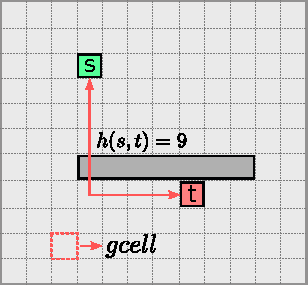
\includegraphics[width=0.35\linewidth]{img/results/problem4/problem4_a.pdf} \label{subfig:problem4_a}}
    \hspace{15pt}
    \subfigure[]{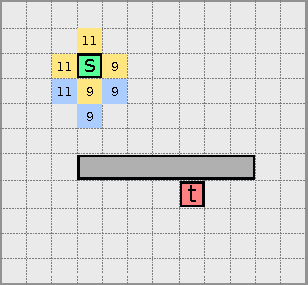
\includegraphics[width=0.35\linewidth]{img/results/problem4/problem4_b.pdf} \label{subfig:problem4_b}} 
    
    \subfigure[]{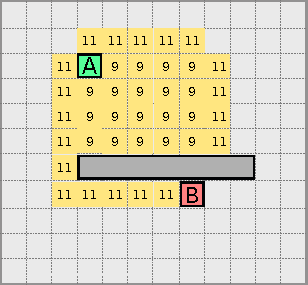
\includegraphics[width=0.35\linewidth]{img/results/problem4/problem4_c.pdf} \label{subfig:problem4_c}}
    \hspace{15pt}
    \subfigure[]{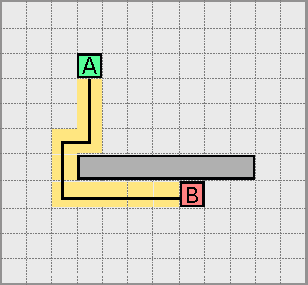
\includegraphics[width=0.35\linewidth]{img/results/problem4/problem4_d.pdf} \label{subfig:problem4_d}}
    
    \caption{Exemplo da execução do algoritmo A*}
    \label{fig:problem4}
\end{figure}

% Para modelar o contexto da etapa de roteamento de \ac{ic} utiliza-se um grafo onde os nodos representam as regiões de roteamento ($gcell$) e as arestas representam as regiões adjacentes.
% Como o leiaute do circuito é subdividido de forma regular e constante é utilizado um modelo de grafo denominado \textit{grid graph}.
Para modelar o contexto da etapa de roteamento global de \ac{ic} utiliza-se um grafo denominado \textit{grid graph}.
Em um \textit{grid graph} todos os nodos adjacentes possuem uma aresta que os interconecta.
Um \textit{grid graph} é definido como $G_{grid} = (V,E)$, onde cada vértice $v \in V$ representa uma $gcell$ e cada aresta $e \in V$ representa as interconexões entre um par de $gcells$ adjacentes ($v_i$, $v_j$).
Para o exemplo ilustrado na Figura~\ref{subfig:problem4_a} será gerado um $G_{grid_{11\times12}}$ com $132$ vértices e $241$ arestas.

% \begin{figure}[ht]
%     \centering
%     \subfigure[]{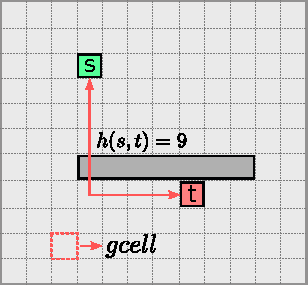
\includegraphics[width=0.35\linewidth]{img/results/problem4/problem4_a.pdf} \label{subfig:problem4_a}}
%     \hspace{15pt}
%     \subfigure[]{\includegraphics[width=0.35\linewidth]{img/results/problem4/problem4_gcell.pdf} \label{subfig:problem4_gcell}} 
    
%     \caption{Exemplo da modelagem do roteamento global.}
%     \label{fig:problem4}
% \end{figure}



% falar que pode rotear com o A*
Uma forma de encontrar o menor roteamento entre dois pinos de uma interconexão (menor caminho no grafo entre as $gcells$ que contêm cada um dos pinos), desviando obstáculos presentes no leiaute do circuito, é o algoritmo A*.
O Algoritmo~\ref{alg:problem4} apresenta um pseudo código para o algoritmo $A^*$ enquanto, a Figura~\ref{fig:problem4} apresenta um exemplo gráfico de sua execução.
Este algoritmo recebe como entrada um vértice fonte $s$ e um vértice destino $t$ (vértices $s$ e $t$ da Figura~\ref{subfig:problem4_a}, respectivamente).
O algoritmo retorna o caminho de menor custo entre $s$ e $t$.

\begin{algorithm}[h!t]
\SetKwInOut{Input}{Entrada}\SetKwInOut{Output}{Saída}
\SetKwRepeat{Do}{do}{while}
\SetKw{Continue}{continue}
\SetKwProg{FReconstructPath}{RECONSTRUCT\_PATH}{}{}
\LinesNumbered
    \Input{source $s \in V$ e target $t \in V$} 
    \Output{caminho de menor custo entre $s$ e $t$}
    $open \gets \{s\}$\; \label{alg:problem4:var:initOpen}
    $closed \gets \emptyset$\; \label{alg:problem4:var:initClosed}
    $g\_score(s) \gets 0$ \; \label{alg:problem4:var:initGscore}
    $f\_score(s) \gets g\_score(s) + h(s, t)$ \; \label{alg:problem4:var:initFscore}
    
    \While{$open \neq \emptyset$}{ \label{alg:problem4:var:initWhileOpen}
        $curr \gets \{c \in open \mid f\_score(c) \leq f\_score(c'), \forall c' \in open \}$ \; \label{alg:problem4:var:initcurr}
        \uIf{$curr = t$}{ \label{alg:problem4:var:IfcurrIsTarget}
            \Return RECONSTRUCT\_PATH($curr$, $s$)\; \label{alg:problem4:var:callReconstructPath}
        }
        $open \gets open - \{curr\}$\; \label{alg:problem4:var:removecurrFromOpen}
        $closed \gets closed \cup \{curr\}$\; \label{alg:problem4:var:aadcurrInClosed}
        \ForEach{ $n \in neighbors(curr)$}{ \label{alg:problem4:var:initForNeighbors}
            \uIf{$n \notin closed \land capacity(curr, n) \geq 1$}{ \label{alg:problem4:var:ifNinClosed}
                $g\_score' \gets g\_score(curr) + w(curr,n)$\; \label{alg:problem4:var:initTentGScore}
                \uIf{$n \notin open \lor g\_score' < g\_score(n)$}{ \label{alg:problem4:var:ifNinOpenORtentScoreLess}
                    $came\_from(n) \gets curr$\; \label{alg:problem4:var:initCameFront}
                    $g\_score(n) \gets g\_score'$\; \label{alg:problem4:var:updatGScoreN}
                    $f\_score(n) \gets g\_score(n) + h(n, t)$ \; \label{alg:problem4:var:updatFScoreN}
                    $open \gets open \cup \{n\}$\; \label{alg:problem4:var:addNinOpen}
                }
            }
        } \label{alg:problem4:var:endForNeighbors}
    } \label{alg:problem4:var:endWhileOpen}
    \Return $\emptyset$ \label{alg:problem4:var:returnEmpty}
    
    \FReconstructPath{($curr \in V$, $s \in V$)}{
        $total\_path \gets [curr]$\;
        \While{$curr \neq s$}{
            $curr \gets came\_from(curr)$\;
            $total\_path.insert(curr)$\;
        }
        \Return $total\_path$\;
    }
    
  \caption{$A^*$} \label{alg:problem4}
\end{algorithm}

\simbolo{$h(s, t)$}{\\ heurística entre as $gcell$ $s$ e $t$}
\simbolo{$g\_score(x)$}{\\ custo para percorrer o caminho entre $s$ e $x$}
\simbolo{$f\_score(x)$}{\\ estimativa do custo total entre $s$ e $t$, que passe pelo vértice $x$}
\simbolo{$neighbors(curr)$}{\\ vértices vizinhos ao vértice $curr$}

A busca do caminho entre os vértices do grafo é baseada em uma busca em largura.
Inicialmente o vértice $s$ é adicionado ao conjunto que contém todos os vértices a serem visitados, chamado de $open$ (linha \ref{alg:problem4:var:initOpen}).
O conjunto $closed$ contém os vértices que foram visitados pelo algoritmo e por este motivo ele é inicialmente vazio (linha \ref{alg:problem4:var:initClosed}).
O algoritmo mantém dois \textit{scores}, $g\_score(x)$ e $f\_score(x)$, para cada vértice pertencente ao grafo. 
A função $g\_score(x)$ representa o custo para percorrer o caminho entre $s$ e $x$.
A função $f\_score(x)$ retorna a estimativa do custo total entre $s$ e $t$, que passa pelo vértice $x$.


% As funções $g\_score(x)$ e $f\_score(x)$ (linhas \ref{alg:problem4:var:initGscore}, \ref{alg:problem4:var:initFscore}, \ref{alg:problem4:var:initTentGScore}, \ref{alg:problem4:var:updatGScoreN} e  \ref{alg:problem4:var:updatFScoreN}) retornam respectivamente o custo do vértice fonte até o vértice $x$; e a estimativa do custo total entre o vértice fonte e o vértice $x$.
Na linha \ref{alg:problem4:var:initFscore}, a função $h(s, t)$ retorna uma estimativa do custo entre dois vértices.
No roteamento global, esta estimativa é realizada através da distância Manhattan entre as $gcell$ representadas pelos vértices.
% Na Figura~\ref{subfig:problem4_a} esta função é definida como $h(A, B)$.

% A cada iteração do laço principal, linha~\ref{alg:problem4:var:initWhileOpen} até \ref{alg:problem4:var:endWhileOpen}, o vértice com menor estimativa do custo total entre ele e o vértice destino $t$ é avaliado.
A cada execução da linha~\ref{alg:problem4:var:initWhileOpen} até \ref{alg:problem4:var:endWhileOpen}, que representa a iteração do laço principal, o algoritmo avalia o vértice que possuir o menor custo, atribuindo-o à variável $curr$ na linha~\ref{alg:problem4:var:initcurr}.
Na Figura~\ref{subfig:problem4_b} o vértice $s$ será o primeiro a ser analisado.
Se o vértice em análise for o próprio vértice destino ($curr = t$) o caminho entre $s$ e $curr$ é reconstruído e retornado pela função RECONSTRUCT\_PATH (linha~\ref{alg:problem4:var:callReconstructPath}).
Se o vértice em análise não for o vértice de destino, então ele é removido do conjunto $open$ (linha~\ref{alg:problem4:var:removecurrFromOpen}) e adicionado no conjunto $closed$ (linha~\ref{alg:problem4:var:aadcurrInClosed}). Isso garante que um vértice só será visitado uma única vez.
% Então, nas linhas~\ref{alg:problem4:var:initForNeighbors} à \ref{alg:problem4:var:endForNeighbors}, para cada vizinho $n$ do vértice $curr$, que não esteja na lista de visitados, é calculado o custo estimado entre $n$ e $t$. Como por exemplo, na Figura~\ref{subfig:problem4_b}, os vizinhos do vértice A estão preenchidos na cor amarela.  Então, o vértice $curr$ é definido como antecessor do vértice $n$ e são atualizados os valores das funções $g\_score$ e $f\_score$ para $n$ (linha~\ref{alg:problem4:var:initCameFront} a  \ref{alg:problem4:var:updatFScoreN}). Caso o vértice $n$ não pertença ao conjunto $open$, o mesmo é adicionado a este conjunto (linha~\ref{alg:problem4:var:addNinOpen}).
Para cada vértice vizinho $n$ ao vértice atual (\textit{curr}) que ainda não foi visitado ($n \notin closed$) e que possuir capacidade de roteamento entre as $gcells$ ($capacity(curr, n) \geq 1$), o algoritmo atualiza os \textit{scores}, o nodo predecessor de $n$ e adiciona $n$ ao conjunto $open$ (linha~\ref{alg:problem4:var:initForNeighbors} a \ref{alg:problem4:var:endForNeighbors}). A função $w(curr, n)$, presente na linha~\ref{alg:problem4:var:initTentGScore}, retorna o custo da aresta entre os vértices $curr$ e $n$.
Na Figura~\ref{subfig:problem4_b}, os vizinhos do vértice $s$ estão preenchidos na cor amarela e seus custos foram atualizados.
Posteriormente à analise do vértice $s$, o vértice abaixo de sua posição será tomado como $curr$ e seus vizinhos (em azul na imagem) serão avaliados.

O algoritmo prossegue nestas iterações até que o vértice $t$ seja encontrado. Caso o conjunto de vértices a serem visitados fique vazio ($open = \emptyset$), o algoritmo retorna um conjunto vazio indicando que não existe caminho possível entre os vértices $s$ e $t$ (linha \ref{alg:problem4:var:returnEmpty}).
A Figura~\ref{subfig:problem4_c} apresenta todos os vértices analisados (em amarelo) e seus respectivos valores, ao passo que a Figura~\ref{subfig:problem4_d} ilustra o caminho retornado pela função  RECONSTRUCT\_PATH para este exemplo.

A função RECONSTRUCT\_PATH recebe como argumento dois vértices e retorna uma lista de vértices pertencentes ao caminho entre estes.
Esta função inicia do vértice $curr$ (que neste caso é o vértice $t$) e iterativamente percorre a lista de vértices predecessores até chegar no vértice $s$.
A função $came\_from(curr)$ fornece o vértice predecessor ao vértice $curr$.
A função $insert(curr)$ insere o vértice $curr$ no início da lista $total\_path$.


\subsection{Modelagem dos Dados}

Para realizar a etapa de roteamento global são necessárias três informações básicas a respeito do \ac{ic}: conjunto das interconexões, conjunto dos pinos pertencentes a cada interconexão e posição dos pinos.
Normalmente, estas informações são divididas em dois módulos: \textit{Netlist} e \textit{Placement}.
Portanto, este estudo de caso utiliza as mesmas informações já apresentadas na Seção~\ref{subsec:modelagemDadosProblem2} para o estudo de caso 2, porém com a modelagem apresentada pela Figura~\ref{subfig:problem2ModelagemDados_OOD} para o modelo \ac{ood} e pela Figura~\ref{fig:problem2Modelagem_DOD_grouped} para o modelo \ac{dod}.
% Como o roteamento utiliza as mesmas informações do que as já apresentadas na Seção~\ref{subsec:modelagemDadosProblem2} do estudo de caso 2, a modelagem das informações para o estudo de caso 4 serão as mesmas apresentadas na Figura~\ref{subfig:problem2ModelagemDados_OOD} para o modelo \ac{ood} e na Figura~\ref{fig:problem2Modelagem_DOD_grouped} para o modelo \ac{dod}.
Note que para o modelo \ac{dod} as propriedades pertencentes aos pinos foram agrupadas pelas interconexões.

A principal diferença entre os estudos de caso 2 e 4 reside no fato de que no estudo de caso 4 é preciso modelar um \textit{grid graph} para representar as informações de roteamento, ao passo que o estudo de caso 2 utilizou uma estrutura de dados simples (elementar).
A Figura~\ref{fig:problem4ModelagemDados} apresenta possíveis modelagens de um grafo para \ac{ood} (a) e \ac{dod} (b).
Os vetores $Edges$ e $Nodes$ na Figura~\ref{subfig:problem4ModelagemDados_DOD} representam as entidades do grafo e os demais vetores representam as propriedades pertinentes a cada uma dessas duas entidades. O vetor $Node Edges$ realiza o mapeamento entre as entidades $Nodes$ e $Edges$ e representa quais arestas um determinado vértice do grafo possui.
Os vetores $w$ e $capacity$ armazenam o peso de cada aresta e suas capacidades, respectivamente.
Para simplificar o problema e garantir a roteabilidade de todas as interconexões, assumiu-se que todas as arestas possuem capacidade infinita de roteabilidade.
Outra simplificação também adotada foi de que todas as arestas possuem o mesmo peso.


\begin{figure}[h!b]
    \centering
    \subfigure[]{\includegraphics[width=0.35\linewidth]{img/results/problem4/gridGraphOOD.pdf} \label{subfig:problem4ModelagemDados_OOD}}
    % \hspace{0.1cm}
    \subfigure[]{\includegraphics[width=0.6\linewidth]{img/results/problem4/problem4_DOD.pdf} \label{subfig:problem4ModelagemDados_DOD}}
    \caption[Organização dos dados estudo de caso 4]{Organização dos dados para modelagem de um grafo segundo os modelos de programação OOD (a) e DOD (b) para o estudo de caso 4.}
    \label{fig:problem4ModelagemDados}
\end{figure}

A Figura~\ref{subfig:problem4ModelagemDados_OOD} apresenta o diagrama de classes para modelagem de um grafo utilizando o modelo \ac{ood}.
As setas com ponta de losango entre as classes representam  uma relação de agregação --- o que significa, por exemplo, que a classe \textit{Grid\_Graph} possui referência para a classe \textit{Node}.
Como já descrito para o modelo \ac{dod}, os atributos $capacity$ e $w$ foram atribuídos igualmente para todas as arestas ($capacity = \infty$ e $w = 1$).


\subsection{Avaliação}

A Figura~\ref{fig:resultsProblem4sequencial} apresenta os resultados da execução sequencial para o estudo de caso 4.
As barras amarelas representam o modelo de dados Orientado a Objetos (\ac{ood}) e as barras azuis representam o modelo Orientado a Dados (\ac{dod}).
À esquerda, na Figura~\ref{fig:missSequentialProblem4}, são apresentados os números de  \textit{cache misses} (eixo Y) para cada circuito avaliado (eixo X).
Para cada circuito, a entrada constituiu-se do conjunto de todas as interconexões e dos respectivos pinos.
À direita, Figura~\ref{fig:runtimeSequentialProblem4}, estão exibidos os tempos de execução (eixo Y), em segundos, para cada circuito avaliado (eixo X).

\begin{figure}[ht]
    \centering
    \subfigure[Número de  \textit{cache misses}.]{\includegraphics[width=0.47\linewidth]{img/results/problem4/problem4_miss_sequential.pdf} \label{fig:missSequentialProblem4}}
    \subfigure[Tempo de execução.]{\includegraphics[width=0.47\linewidth]{img/results/problem4/problem4_runtime_sequential.pdf} \label{fig:runtimeSequentialProblem4}}
    \caption{Resultados para a execução sequencial do estudo de caso 4.}
    \label{fig:resultsProblem4sequencial}
\end{figure}

% \begin{figure}[ht]
%     \centering
%     \includegraphics[width=0.65\linewidth]{img/results/problem4/problem4_miss_sequential.pdf}
%     \caption[Cache misses do Problema~4 sequencial.]{Número de cache misses resultantes dos dois protótipos de software do Problema~4 com execução sequencial.}
%     \label{fig:missSequentialProblem4}
% \end{figure}

% \begin{figure}[ht]
%     \centering
%     \includegraphics[width=0.65\linewidth]{img/results/problem4/problem4_runtime_sequential.pdf}
%     \caption[Tempo de execução Problema~4 sequencial]{Tempo de execução para o Problema~4 com execução sequencial.}
%     \label{fig:runtimeSequentialProblem4}
% \end{figure}

% dados estatísticos
A execução do estudo de caso 4 com o modelo \ac{ood} gerou um número de  \textit{cache misses} de $709M$ a $2709M$ sendo, em média, de $1.33M$ com desvio padrão médio de $0.55\%$ de sua média. 
A execução com o modelo \ac{dod} gerou um número de  \textit{cache misses} de $401M$ a $1008M$ sendo, em média, de $629M$ com desvio padrão médio de $0.79\%$ de sua média.
Isso gerou uma diferença relativa média de $52.81\%$ entre os modelos.
% discussão de ocorrido
É possível observar que houve uma grande redução no número de  \textit{cache misses} com o modelo \ac{dod} se comparado ao modelo \ac{ood} para todos os circuitos.
Para ambos os casos, o circuito com maior número de  \textit{cache misses} foi o \textit{superblue10}.
Isto se deve ao fato deste circuito possuir a maior área dentre todos os circuitos avaliados.
A área é uma característica importante uma vez que ela determina quantas \textit{gcells} serão necessárias para cobrir todo o leiaute do \ac{ic}.
Portanto, como cada vértice do grafo representa unicamente uma \textit{gcell}, este circuito resulta no grafo com maior número de vértices dentre todos os circuitos avaliados.

A redução no número de  \textit{cache misses}, pelo modelo \ac{dod}, é refletida nos tempos de execução.
Este modelo foi mais rápido para todos os circuitos, executando entre $8$ e $22$ segundos e tendo tempo médio de execução de $13.65$ segundos.
O modelo \ac{ood} executou entre $10$ e $38$ segundos, levando em média $19.57$ segundos.
Novamente, assim como no número de  \textit{cache misses}, o circuito \textit{superblue10} foi o que exigiu o maior tempo de execução.
Estes resultados mostram que aplicar o modelo \ac{dod} para representar um grafo é vantajoso e proporciona uma melhoria tanto no acesso aos dados quanto no tempo de execução das aplicações.
Portanto, outras etapas da síntese física que podem ser modeladas com o uso de grafo (como por exemplo a \ac{sta}) devem possuir comportamento similar ao apresentado por este estudo de caso.

Para este estudo de caso não foi implementado uma versão paralela pois sua paralelização não é trivial.
Para realizar o roteamento de duas interconexões $i_1$ e $i_2$ em paralelo seria necessário garantir que o conjunto de $gcells$ pertencente ao roteamento de $e_1$ fosse disjunto do conjunto de $gcell$ do roteamento de $e_2$.
Isto se faz necessário para que as capacidades das $gcells$ sejam atualizadas corretamente e um roteamento não influencie os \textit{scores} ($f\_score$ e $g\_score$ são armazenados nos vértices do grafo) de outro roteamento.